\documentclass[12pt,twocolumn]{article}

% Page dimensions
\setlength{\hoffset}{-0.4in}
\setlength{\voffset}{-0.5in}
%\setlength{\headsep}{-0.2in}
\setlength{\oddsidemargin}{0in}
\setlength{\textwidth}{7.4in}
\setlength{\textheight}{8.5in}
\setlength{\columnsep}{0.3in}

% Packages
\usepackage{fancyhdr}
\usepackage{abstract}
\usepackage{amsmath,amssymb} 
\usepackage{subcaption} 
\usepackage[usenames,dvipsnames]{color}
\usepackage{placeins}
\usepackage{hyperref}
\usepackage{sectsty}
\usepackage{enumitem}
\usepackage{todonotes}
\usepackage{lastpage}

\hypersetup{
	colorlinks=false,
	pdfborder={0 0 0},
}

%\usepackage[inline]{showlabels}
%\showlabels[\color{blue}]{cite}
%\showlabels[\color{blue}]{ref}

%% ============================================================

% Macros
%\newcommand{\CHRONO}{{\sffamily{{Chrono}}}}
%\newcommand{\ChronoFEA}{{\sffamily{Chrono}}::FEA}
%\newcommand{\ChronoVehicle}{{\sffamily{Chrono}}::Vehicle}
%\newcommand{\ChronoFSI}{{\sffamily{Chrono}}::FSI}
%\newcommand{\ChronoGranular}{{\sffamily{Chrono}}::Granular}
%\newcommand{\ChronoParallel}{{\sffamily{Chrono}}::Parallel}
%\newcommand{\ChronoDistributed}{{\sffamily{Chrono}}::Distributed}
%\newcommand{\ChronoOpenGL}{{\sffamily{Chrono}}::OpenGL}

\newcommand{\chrono}{Chrono}
\newcommand{\chronomod}[1]{\chrono{}::#1}
\newcommand{\synchrono}{Syn\chrono{}}
\newcommand{\gymchrono}{Gym\chrono{}}
\newcommand{\pychrono}{Py\chrono{}}

\newcommand{\gps}{\textsc{gps}}
\newcommand{\imu}{\textsc{imu}}
\newcommand{\mpi}{\textsc{mpi}}
\newcommand{\lidar}{lidar}
\newcommand{\cpu}{\textsc{cpu}}
\newcommand{\dsrc}{\textsc{dsrc}}
\newcommand{\gpu}{\textsc{gpu}}
\newcommand{\ros}{\textsc{ros}}
\newcommand{\tcp}{\textsc{tcp}}
\newcommand{\fea}{\textsc{fea}}
\newcommand{\api}{\textsc{api}}
\newcommand{\scm}{\textsc{scm}}
\newcommand{\optix}{OptiX}

%% ============================================================

% Styles

\definecolor{my-gray}{gray}{0.4}

% First page header
\fancypagestyle{firststyle} {
	\lhead{}
	\rhead{
	\footnotesize
	\textbf{2020 NDIA GROUND VEHICLE SYSTEMS ENGINEERING AND TECHNOLOGY SYMPOSIUM}\\
	\textbf{\sc Autonomy, Artificial Intelligence \& Robotics (AAIR) Technical Session}\\
	\textbf{\sc August 11-13, 2020 -- Novi, Michigan}	
	}
	\chead{}
	%
	\lfoot{}
	\cfoot{}
	\cfoot{\footnotesize DISTRIBUTION STATEMENT A. Approved for public release; distribution unlimited. OPSEC\#864}
	\rfoot{}
}

% All other pages (header and footer)
\pagestyle{fancy}
\fancyhf{}
\rhead{
	\color{my-gray}
	\footnotesize Proceedings of the 2020 Ground Vehicle Systems Engineering and Technology Symposium (GVSETS)
	}
\cfoot{
	\color{my-gray}
	\footnotesize
	{\FooterTitle}\\
	Page \thepage~of~\pageref{LastPage}
}

\renewcommand{\headrulewidth}{0pt}

% Font and styles for sections
\allsectionsfont{\fontsize{12}{15}\selectfont}

\renewcommand{\abstractname}{ABSTRACT}
\renewcommand{\refname}{REFERENCES}

%% ============================================================


\newcommand{\todo}[1]{\textcolor{red}{\textbf{#1}}}

% highlighting, coloring, etc.
\newcommand{\highlightThis}[1]{\textcolor{red}{{\bf{{#1}}}}}
\newcommand{\highlight}[1]{\textcolor{red}{#1}}
\newcommand{\textcolorRED}[1]{{\textcolor{red}{#1}}}
\newcommand{\textcolorBLACK}[1]{{\textcolor{black}{#1}}}


\newcommand{\softpackage}[1]{{\sffamily{#1}}}
\newcommand{\CHRONO}{{\softpackage{{Chrono}}}}

\newcommand{\sbelNewSolution}[1]{\medskip\noindent{\textit{#1}}}

\newcommand{\gonogo}{{\normalfont\textsc{go/no-go}}\xspace}
\newcommand{\go}{{\normalfont\textsc{go}}\xspace}
\newcommand{\nogo}{{\normalfont\textsc{no-go}}\xspace}
%\newcommand{\chrono}{{\textsl{Chrono}}\xspace}

\newcommand{\Reg}{\textsuperscript{\tiny\textregistered}}

\newcommand{\papertitle}{Enabling Artificial Intelligence Studies in Off-Road Mobility Through Physics-Based Simulation of Multi-Agent Scenarios}

%% ============================================================

\title{\bf\large \MakeUppercase{\papertitle{}}}

\newcommand{\FooterTitle}{\papertitle{}, Negrut, et al.}

\author{	
	{\bf D. Negrut, R. Serban, A. Elmquist, J. Taves, A. Young}\\
	University of Wisconsin -- Madison\\
	Madison, WI
	\and
	{\bf A. Tasora, S. Benatti}\\
	Dipartimento di Ingegneria ed Architettura \\
	University of Parma, Italy
}

\newcommand{\MyAbstract}{\textit{
\noindent 
We describe a simulation environment that enables the designing and testing of control policies for off-road mobility of autonomous agents. Herein, the environment is used in conjunction with the design and demonstration of a reinforcement learning generated policy that uses sensor fusion and inter-agent communication to enable the movement of mixed convoys of conventional and autonomous vehicles. Policies learned on rigid terrain are shown to transfer to hard (silt-like) and soft (snow-like) deformable terrains. The enabling simulation environment, which is Chrono-centric, is used as follows: the training occurs in the GymChrono learning environment using PyChrono, the Python interface to Chrono. The GymChrono-generated policy is subsequently deployed for testing in SynChrono, a scalable, cluster-deployable multi-agent testing infrastructure that uses MPI. The Chrono::Sensor module simulates sensing channels used in the learning and inference processes. The software stack described is open source. Relevant movies: \cite{simsPaperGVSETS2020}.
} 
}




%% ============================================================

\begin{document}
\date{}

% ------------------------------------------

\twocolumn[
\maketitle             % full width title
\thispagestyle{firststyle}
\begin{onecolabstract} % ditto abstract
\MyAbstract
\end{onecolabstract}
\vspace{0.1in}
]

\newpage

%% ============================================================

\section{INTRODUCTION}
\label{s:introduction}
Computer simulation has been extensively used in the design and analysis of various automation aspects tied to on-road mobility, see, for instance \cite{carlaAVsim2017}. A similar statement cannot be made for off-road mobility owing to a smaller market and a set of stiff challenges brought along by the task at hand. However, a predictive simulation platform for off-road mobility analysis of autonomous agents (AAs) is very desirable since it can accelerate the engineering design cycle, reduce costs, perform more thorough testing, and produce more performant and safer designs. Simulation is not a silver bullet as it has its limitations, first of all the issue of simulation-to-reality transfer \cite{sim2realGapEssex1995}, which pertains to the failure of control policies derived in simulation to work well in the real world. Furthermore, models are difficult to set up and calibrate, the validation process can be tedious and time consuming, and simulation tools that are both predictive and expeditious are not available for all types of analysis. This contribution addresses the third point. It describes a simulation environment whose stated purpose is to allow the practitioner to gain insights into the operation of AAs (robots and autonomous wheeled or tracked vehicles) in off-road conditions. If such a simulation platform is validated, it can be used to two ends: produce mechanical design of AAs; and generate and test control policies that govern the operations of the AAs.

There are many other ongoing efforts that seek to address the AA simulation issue. In robotics, Gazebo~\cite{gazebo,koenig2004design} is a widely used 3D multi-robot simulator with dynamics.  It is not a simulation engine per se, but a \textit{platform} that exposes several engines: ODE~\cite{ode2015}, Bullet~\cite{bulletPhysicsEngine2020}, DART~\cite{dart2018}, and Simbody~\cite{sherman2011simbody}. Unlike Gazebo, which is open source, CoppeliaSim (formerly V-REP)~\cite{V-REP2013} is a commercial multi-robot simulation solution that also exposes a set of simulation engines: MuJoCo~\cite{todorovMujoco2012}, Vortex Dynamics~\cite{cmLabs2020}, Bullet, and Newton Dynamics~\cite{newtonDynamics2020}. ROAMS~\cite{abhiROAMS2004} and ANVEL~\cite{ANVEL-website} are two other simulation engines for off-road AAs. The former is used for mission planning by NASA and draws on an in-house dynamics engine~\cite{DARTS}; the latter relies on the ODE simulation engine and has been used in the past for off-road military applications~\cite{ANVELdescription2012} in combination with a sensor simulation package~\cite{VANE-2012}. MAVS is an off-road AA simulation environment that is currently under active development \cite{mavsCarruth2018}. It provides an in-house developed, sophisticated sensor simulation module \cite{goodin2018enabling,goodin2019predicting}, has a ROS bridge, and uses Chrono as its dynamics engine. USARSim is an AA simulation platform, not under active development, that draws on a game engine (Unreal Engine~\cite{unrealEngine}), a choice with pluses (scalability, ability to create complex worlds) and minuses (the simulation engine is designed for plausibility rather than accuracy). For autonomous vehicle (AV) simulation, Carla~\cite{carlaAVsim2017} and AirSim~\cite{shah2018airsim} are two often used open-source simulators, the former for on-road AV driving scenarios simulation, the latter originally designed for drones but now including support for on-road traffic of AVs as well. Carla and AirSim rely on Unreal Engine but several other engines are used for AA simulation, e.g. Unity~\cite{unityGaming} and TORCS~\cite{torcsRacingSimulation2020}. For a survey of other solutions for on-road mobility the user is referred to~\cite{surveyAVsimulationBerger2019}.

The AA off-road mobility simulation platform discussed here is Chrono-centric~\cite{projectChronoWebSite,chronoOverview2016}. In its purpose, it is similar to the ANVEL-VANE environment as it seeks to simulate robots and wheeled/tracked vehicles operating in off-road conditions. Compared to the ANVEL-VANE solution, the Chrono environment is different in several respects: it is open source and available for unfettered use under a BSD3 license, it uses its own multi-physics engine, it is scalable and deployable on supercomputers, clusters, or multi-core architectures owing to its reliance on the MPI message passing standard for parallel computing~\cite{MPI-Forum-1994}, and is under active development. Chrono is an ecosystem of modules and toolkits. It has support for rigid and flexible body dynamics (Chrono::Engine), fluid-solid interaction (Chrono::FSI), and granular dynamics (Chrono::Parallel and Chrono::Granular) applications. It has Python bindings, support for sensor simulation in Chrono::Sensor, an API for interaction with ROS~\cite{ROS-2009}, as well as facilities for: rapid vehicle modeling via parameterized templates~\cite{ChronoVehicle2019}; control policy design with GymChrono; and scalable control policy testing with SynChrono. Chrono relies on GPU computing for fluid-solid interaction and some granular dynamics simulations, multi-core for most of the other modules, and MPI-enabled parallel computing for co-simulation when handling large terramechanics applications or collections of AAs. Real-time simulation is not one of Chrono's priorities. Although as shown in this contribution, for simple robotics or vehicle-on-rigid-road simulation it provides faster than real-time performance, there are numerous applications that lead to long run times, e.g., deformable terrain mobility, nonlinear flexible body dynamics, fording scenarios, etc. 

This contribution highlights the Chrono components that support the design and testing of control policies through simulation: PyChrono, GymChrono, Chrono::Sensor, and SynChrono. To show these components at work, a Reinforcement Learning (RL) approach is used herein to produce a control policy. There is nothing special about the RL approach; other techniques to design control policies could be used equally well, a point touched upon in more detail in Section \S\ref{sec:ML}. Section \S\ref{sec:simInfrastructure} describes the Chrono infrastructure that facilitates artificial intelligence studies in off-road, multi-agent mobility scenarios. Section \S\ref{sec:demoTechnology} covers simulation experiments that highlight two aspects: the scalability of the SynChrono testing environment, and the process of designing the RL control policy along with an evaluation of the policy's robustness. Concluding remarks and directions of future work round off the contribution. 



\section{DERIVING CONTROL POLICIES THROUGH SIMULATION}
\label{sec:ML}
Derived using an accurate and robust simulation framework, controls algorithms have shown to carry over to real-life successfully~\cite{VISTASimMITRL, VirtualToRealRL}. The use of vehicles with Level 1 and Level 2 autonomy has grown considerably~\cite{J3016_201401, SAEHardwareInTheLoop} and the automotive industry is making major strides towards producing Level 3 and Level 4 vehicles~\cite{WayveRLSimToReal, TeslaSummon}. Owing to advantages already described, the use of simulation in the on-road AV sector is an area of intense research and development. A common solution to the AV control problem relies on sampling-based methods. These approaches generate many candidate trajectories a vehicle can follow, selecting and executing the controls associated with the best candidate~\cite{UrbanAVBezierMPC, RRTRealTime}. Consequently, they require a discrete state space. Graph search methods are commonly associated with each trajectory. In general, this approach is real-time challenged, as achieving robust results requires a high number of samples to be analyzed~\cite{TrajectoryPlanningMIQP}. Algorithms such as Dijkstra's, A-Star (A*), or the Rapidly-exploring Random Tree-Star (RRT*), sample the state space either deterministically or stochastically~\cite{RRTRealTime}. Depending on the complexity of the traffic scenario, these algorithms can prove computationally costly and provide sub-optimal results.

Model Predictive Control (MPC) is another common AV control approach in which a continuous state space is used~\cite{Borrelli2005MPCbasedAT}. Using a dynamic model of a vehicle, the MPC algorithm computes trajectories over the state space and determines an optimal trajectory using gradient-descending optimization techniques~\cite{TrajectoryPlanningMIQP, Liniger2017OptimizationBasedAR}. A limited time horizon is employed to reduce unneeded computation for times too far out into the future. In comparison to sampling algorithms, the MPC approaches show improved performance that is tied to the use of the gradient fields in the optimization problem that comes into play~\cite{Borrelli2005MPCbasedAT}.

The accuracy of the simulation platform plays a critical role for MPC as well as sampling-based controllers. To adequately validate and subsequently verify a controller such as MPC, the simulation must be of high enough definition to carry over successfully to reality~\cite{AVTestingMethods}. Likewise, for PID controller solutions, for which gains must be carefully selected, an inaccurate simulation platform could yield a poor design that leads to undesired consequences when deployed on a real vehicle.

The design of a robust controller that performs adequately in complex environments using the aforementioned strategies has proven difficult when aiming for a generalized policy~\cite{Kuutti2019ASO}. An emerging approach that has gained momentum in recent years is Machine Learning (ML) based \cite{surveyRLrobotics2013}. ML has shown promise in producing efficient and robust models that generalize well in a variety of situations. The three pillars of ML include supervised learning, unsupervised learning, and reinforcement learning. In the AA problem, deep reinforcement learning (DRL) has been very successful, as it displays the ability to learn and respond in complex scenarios without the need for preprocessed or labeled data~\cite{VirtualToRealRL}.

Since its introduction~\cite{Mnih13}, DRL has proven successful in continuous control applications of robots~\cite{Levine2016,inHandManipulation2020}. At its core, DRL is an iterative learning process in which an \emph{agent} interacts with an \emph{environment}; at each iteration the agent collects an \emph{observation} (or \emph{state}), then performs an \emph{action} based on the previous observation and gets a \emph{reward} which is a measure of its performance. The goal of RL is finding a policy that maximizes the sum of the collected reward. In a broad sense, a policy prescribes an action given a state.

RL allows for complex control policies viable in unstructured and stochastic environments; it is model-free in that it does not require a model that predicts the environment transition; and can learn from scratch. RL's major flaw is its need for a massive amount of training data to infer a robust policy. The role of simulation is to produce this collection of samples. \emph{Policy Gradient Algorithms} are a subset of RL algorithms whose goal is to directly learn an optimal stochastic policy $\pi_\theta(a|s)$, where $s$, $a$, and $\theta$ are the state, action, and a set of learnable parameters, respectively. If $\pi$ is a Neural Network (NN), $\theta$ are the weights and biases of the NN, the state is the NN input, and the action is its output. Proximal Policy Optimization (PPO)~\cite{Schulman2017PPO} is one of the most widely used algorithms for continuous state and action environments and is the algorithm of choice for this demonstration. PPO is a policy gradient algorithm whose goal is to optimize a stochastic policy. It is also an actor-critic method since another NN is trained and used to estimate the Value Function~\cite{SuttonBarto1998RL} employed to estimate the Advantage Function~\cite{Kakade02approximatelyoptimal}. The Advantage Function is used in the objective function to be maximized.

\section{SIMULATION INFRASTRUCTURE}
\label{sec:simInfrastructure}
The purpose of the simulation environment described is twofold. First, it is used to produce the data needed to design a control policy. Second, it is used for testing purposes; i.e., exposes the control policy that was produced in a model-based or model-free approach to a battery of tests to gauge its correctness and robustness. This section outlines the components of this Chrono-centric simulation environment. The emphasis is placed on four components: Chrono::Sensor, PyChrono, GymChrono and SynChrono, that anchor the AA design and testing process and have not been discussed elsewhere in detail. Other Chrono components or functionality will be touched upon in passing since they have been described elsewhere \cite{chronoOverview2016,ChronoVehicle2019,ChronoSCM2019}.

\paragraph{Chrono.} Under active development for over two decades, Chrono~\cite{chronoOverview2016} is a multi-physics simulation engine distributed as open-source under a permissive BSD license.  Its core module, Chrono::Engine, provides support for rigid multibody dynamics, nonlinear finite element analysis, and frictional contact dynamics. Chrono is modular, with optional modules providing support for additional classes of physics simulation (e.g., fluid-solid interaction or large-scale granular dynamics), for modeling and simulation of specialized mechanical systems (e.g., ground vehicles), for interfaces to external solvers (e.g., sparse direct linear solvers), or for dedicated parallel algorithms targeting different computing architectures (multi-core, distributed, and GPU) for large-scale simulations.

Written almost entirely in C++, Chrono is middleware and therefore supports customized solutions that involve user code and potentially third-party software. The software is portable and can be built on different platforms, under different operating systems, and using various compilers. Chrono is actively developed, has a continuous integration process, an active user forum, and is managed through GitHub~\cite{projectChronoGithub}; it's latest release is 5.0.1, available as of March 2020.  Chrono is used by academic, industrial, and government research and development groups and projects.

\paragraph{Chrono::Vehicle.} Chrono::Vehicle~\cite{ChronoVehicle2019} is a specialized Chrono module which provides a collection of templates (parameterized models) for various topologies of both wheeled and tracked vehicle subsystems. It also provides support for modeling of rigid, deformable, and granular terrain, support for closed-loop and interactive driver models, and run-time and off-line visualization of simulation results. Chrono::Vehicle leverages and works in tandem with other Chrono modules for run-time visualization or finite element, granular dynamics, and parallel computing support.

Chrono::Vehicle provides a comprehensive set of vehicle subsystem templates (for tires, suspensions, steering mechanisms, drivelines, sprockets, track shoes, etc.), templates for external systems (powertrains, drivers, terrain models), and additional utility classes and functions for vehicle visualization, monitoring, and collection of simulation results.  As a middleware library, Chrono::Vehicle requires the user to provide C++ classes for a concrete instantiation of a particular template.  An optional Chrono library provides complete sets of template instantiations for several concrete ground vehicles, both wheeled and tracked, which can serve as examples for developing more customized vehicle models. An alternative mechanism for defining concrete instantiation of vehicle system and subsystem templates is based on input specification files in the JSON format.  For additional flexibility and to allow integration of third-party software, Chrono::Vehicle is designed to permit either monolithic simulations or co-simulation where the vehicle, powertrain, tires, driver, and terrain/soil interaction can be simulated independently.

\begin{figure}
    \centering
    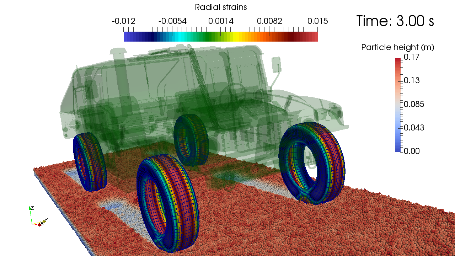
\includegraphics[width=0.8\columnwidth]{Figs/HMMWV-Granular.png}
    \caption{{\small Chrono::Vehicle HMMWV with flexible tires navigating granular terrain demonstrating vehicle dynamics, flexible body dynamics, and parallel computing support in Chrono \cite{antonioVehicleTireGranMatSim2017}.}}   
    \label{fig:hmmwvgranular}
\end{figure}

Chrono::Vehicle provides several classes of terrain and soil models, of different fidelity and computational complexity, ranging from rigid, to semi-empirical Bekker-Wong type models, to complex physics-based models based on either a granular or finite-element based soil representation.  For simple terramechanics simulations, Chrono::Vehicle provides a customized implementation of the Soil Contact Model (SCM), based on Bekker theory, with extensions to allow non-structured triangular grids, adaptive mesh refinement, and incorporation of bulldozing effects~\cite{ChronoSCM2019}.  Second, Chrono provides an FEA continuum soil model based on multiplicative plasticity theory with Drucker-Prager failure criterion and  specialized brick elements. Finally, leveraging Chrono support for large-scale granular dynamics and for multi-core, GPU, and distributed parallel computing, off-road vehicle simulations can be conducted using fully-resolved, granular dynamics-based complex terramechanics, using a Discrete Element Method approach, see Fig.~\ref{fig:hmmwvgranular} \cite{antonioVehicleTireGranMatSim2017, serbanCosimIJVP2019}.


\paragraph{Chrono::Sensor.} Chrono::Sensor is a specialized module of Chrono that enables the modeling and simulation of sensors for simulating robots and autonomous vehicles for software-in-the-loop testing. This module allows for cameras, lidar, GPS, and IMU sensors to be placed within a Chrono simulation to generate synthetic data based on user-defined sensor parameters. The goal of the module is to allow realistic data generation based on sensor characteristics such as noise, distortion, and lag. Sensors can be attached to objects within the simulation and configured to match corresponding real sensors. For ease of modeling, sensors can be specified through a JSON file format. Additionally, custom sensors and post-processing filtering can be implemented leveraging the existing render framework or physics interface. 

For interoceptive sensing (GPS and IMU), the module utilizes the internally computed physical quantities from the Chrono system and can augment this ground truth with drift, Gaussian noise, lag, and collection time. For exteroceptive sensors that provide information about scene characteristics (camera and lidar), Chrono::Sensor leverages hardware accelerated ray tracing through the OptiX library~\cite{optixNVIDIA} and implements physically based rendering techniques. The ray tracing approach allows for the physical reconstruction of the light-based data acquisition process and thus controls the attributes of the synthetically generated sensor data. For camera, lens models and post-processing noise augmentation are supported, with an interface to extend or implement custom models. For lidar, the framework expands on work from~\cite{goodin2018enabling} to provide a beam divergence model that can support multiple modes of lidar return and reduced intensity during partial beam reflectance. 

Chrono::Sensor is currently in development with planned expansion of sensor support and additional distortion model implementations. All sensors and capabilities are written in C++, but can also be accessed from Python through the PyChrono interface. The entire module can be run headless without the requirement of a render context, allowing for ease of deployment in machine learning applications on remote servers.


\paragraph{PyChrono.} While the main Chrono API is C++, in recent years a concerted effort was dedicated to providing automatically-generated Python wrappers for much of the Chrono functionality. The main rationale for this was providing a lower-entry point to modeling and simulation with Chrono for users less familiar with C++ but also, as importantly, providing an interface to various machine learning platforms, such as TensorFlow \cite{tensorflow}, PyTorch \cite{paszke2017PyTorch}, Theano \cite{theano2016}, and CAFFE \cite{caffe2014}.  

The Python wrapping relies on using automated technology provided by SWIG, which generates the interface between Python user-code and the underlying Chrono C++ libraries.  As of today, a large set of Chrono functionality is exposed to Python users, including the core multibody and FEA module, the interface to CAD systems (like SolidWorks), run-time visualization with Irrlicht, etc. In particular, full support is available for both modeling, simulation, and visualization of wheeled ground vehicles and use of the Chrono::Vehicle existing wheeled vehicle models, as well as using the sensor models provided by Chrono::Sensor. PyChrono for Python 3 can be built from sources on any of the supported platforms (Linux, Windows, MacOS).  Alternatively, pre-built conda PyChrono packages are available on the project's Anaconda page~\cite{pyChronoCondaWebSite} (note that Chrono::Sensor is not available yet via the conda PyChrono packages). 

\paragraph{GymChrono.} GymChrono is an extension of OpenAI Gym~\cite{Brockman16Gym}. It exposes a set of environments providing continuous control tasks for physics and sensor simulation run by the Chrono backend. These environments inherit from OpenAI Gym classes. As such, they can be used out of the box with any algorithm or DRL framework made for gym environments; and, they can draw on gym's environment parallelization for learning acceleration.

\paragraph{SynChrono.} SynChrono is a software component that uses Chrono to implement a distributed-memory execution model when simulating scenarios that include multiple AAs. It leverages the Message Passing Interface (MPI) standard~\cite{mpi-3.0}, which allows the toolset to have multiple instances of Chrono run simultaneously on a supercomputer, cluster, or multi-core setup to allow for the distributed simulation of multiple agents (robots, tracked vehicles, wheeled vehicles, etc.) The paradigm embraced is that of running one Chrono agent simulation as one MPI rank, with multiple ranks communicating through MPI messages to maintain a space and time coherent solution for all agents participating in the study. As an example, if there are two agents, SynChrono makes it possible to synchronously run the two agents on two different compute nodes in a supercomputer. By the same token, if there are 50 agents and 50 compute nodes in a cluster, SynChrono provides the compute infrastructure to keep the 50 agents operating in a coherent (timewise and spacewise) virtual world. Although each agent represents a Chrono simulation, SynChrono makes it possible for ruts generated by agent 27 to be picked up on a camera sensor on agent 31 if the camera points to agent 27. The time coherence aspect prevents some agents from racing into the future while other agents lag behind in the past. The global synchronization mechanism in SynChrono ensures that all 50 agents march forward in simulation time in a coherent fashion so that mutual interaction (a vehicle crossing the ruts of a different one, a vehicle sensing another vehicle, etc.) happens as in real life.

The structure of SynChrono's MPI framework is shown in Fig.~\ref{fig:mpischematic}. Each agent runs in its own MPI rank and interfaces with its dedicated control stack for software-in-the-loop control. The control stack is fed synthetic data generated by Chrono::Sensor and acts upon the environment through Chrono::Vehicle control inputs (throttle, steering, braking). This ``one agent-to-one Chrono system'' mapping ensures scalability; a monolithic Chrono system could not deliver this, a point demonstrated in section \S\ref{sec:demoTechnology}. The control algorithm for each agent is also configurable and can vary from complex algorithms that fuse a variety of sensor data streams, to controls based on empirical models, and on to pre-recorded driver inputs from a human or human-driven control in scenarios that are simple enough to allow real-time simulation (SynChrono supports human-in-the-loop experiments). 

\begin{figure}
	\centering
	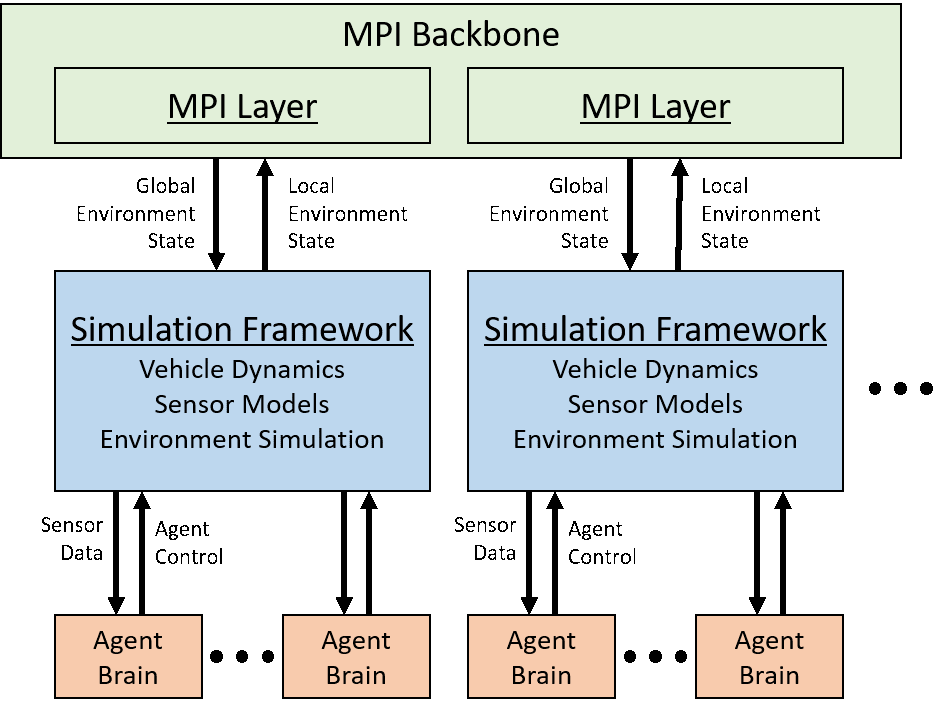
\includegraphics[width=\columnwidth]{Figs/MPI-schematic.png}
	\caption{{\small Schematic of the SynChrono framework. Decisions are passed to the Chrono system for dynamics simulation and the outcome of the dynamics simulation is synchronized between ranks using MPI.}}   
	\label{fig:mpischematic}
\end{figure}

Each MPI rank is responsible for the dynamics of a single agent and simulates those dynamics as if that agent were the only agent in the world. At a slow frequency (relative to the simulation time-step), all ranks communicate with a central controller to exchange state information. State information is intended to be brief, communicating the bare minimum of information to enable other ranks to reconstruct a visual-only version of the agent in their own world. In an example where each agent is a vehicle, the state information consists of the vehicle location and orientation along with pose information for each wheel. This information is packaged via the FlatBuffers serialization library \cite{flatbuffers}. This allows a rank receiving this state information to construct a visual copy in their world for visualization or sensing purposes. SynChrono can add additional agents to the simulation at almost no extra cost, the only overhead being a higher volume of messages moving on the network and through the central controller. 

One limitation of the implementation is that currently two agents running as two different Chrono processes (ranks) cannot crash with each other or participate in an operation that couples their dynamics, e.g. lifting together a heavy object. Such a scenario should be run in Chrono, since the coupling is too tight to be handled by SynChrono. This will make the simulation longer to run since more agents will have to be handled within one rank (Chrono process). However, if the agent coupling happens via sensing or the virtual world, e.g., one agent sensing another one, one vehicle crossing over and being jolted by the ruts left by a different agent, then SynChrono can be relied on, thus ensuring scalability. The goal of SynChrono is to have virtually constant scaling up to a high threshold where high message volume dominates over the dynamics computation. 

\paragraph{Interface to an external controller.} For testing of control algorithms that are intended to be easily transferred to real-life vehicles or robots, the simulation platform provides an external control interface that is exposed in SynChrono. An agent in SynChrono can send messages (i.e. sensor data packets) to the external autonomous controls framework which can then send a message back (i.e. control inputs). The control stack is independent of the SynChrono platform (i.e. a bridge has been developed for ROS \cite{ROS-2009}), and can be tested with inputs replicating those from reality, such as sensor and/or V2X communication data.

%% ===========================================================
\section{TECHNOLOGY DEMONSTRATION}
\label{sec:demoTechnology}


\subsection{SynChrono scaling analysis}\label{sec:syn-scaling-analysis} 
SynChrono is an environment that uses $N+1$ processes executing on a cluster/supercomputer to simulate the dynamics of $N$ agents handled as $N$ independent Chrono simulation. Each Chrono simulation is a process; the extra compute node is involved in maintaining the time and space coherence for the virtual world shared by the $N$ agents. The so-called SynChrono daemon executes as the extra process and it manages through MPI the dynamics of the $N$ agents. The numerical experiments described here answer the following questions: ($i$) How does the time to complete a simulation change as $N$ increases? ($ii$) How fast is SynChrono in mobility studies on rigid terrain? ($iii$) How fast is it when an SCM deformable terrain model is considered in the simulation scenario? These experiments were conducted with up to $N=14$ agents, using rigid, SCM hard (silt-type), and SCM soft (snow-like) terrain.  

The handling of a virtual world that has SCM terrain is challenging since each of the $N$ vehicles changes the terrain at the same time and these changes must be space and time coherent. This is facilitated and managed by the SynChrono daemon. The key component of the SCM terrain is the deformation of each vertex in the underlying SCM mesh. All other terrain properties can be computed based on the height of each vertex alone~\cite{ChronoSCM2019}. At each simulation step, a SynChrono rank that is associated with an agent moving on SCM terrain collects a list of the deformed vertices that the agent produced during the course of that time step. Mesh deformation data may not be sent at every simulation time-step, so this collection of mesh changes is in general persistent across simulation time steps. Once an agent reaches a SynChrono synchronization point, the cumulative mesh deformations produced by one agent are sent via the daemon to every other agent's world. Each agent then applies the deformations to their own copy of the SCM mesh and resets their collection of new mesh deformations. This means that two agents should not come close enough that they deform the same vertices during the same synchronization period, but this is just as restrictive as SynChrono's assumption that any two agents will not interact by crashing. While Chrono's SCM implementation allows for meshes that auto-refine, this is currently not supported in SynChrono due to the significant increase in algorithmic complexity for little gain in performance. The main concern for scalability is message size, since for synchronizing SCM terrain there is about 15 times as much data to send for each agent relative to the rigid terrain case. 

The scenario discussed herein is that of many vehicles crossing perpendicularly on a rectangular patch of SCM terrain, shown in Fig.~\ref{fig:scalingenv}. This scenario allows for easily scaling up the number of vehicles and verifying that the SCM terrain deformation is properly synchronized across multiple ranks.

\begin{figure}
    \centering
    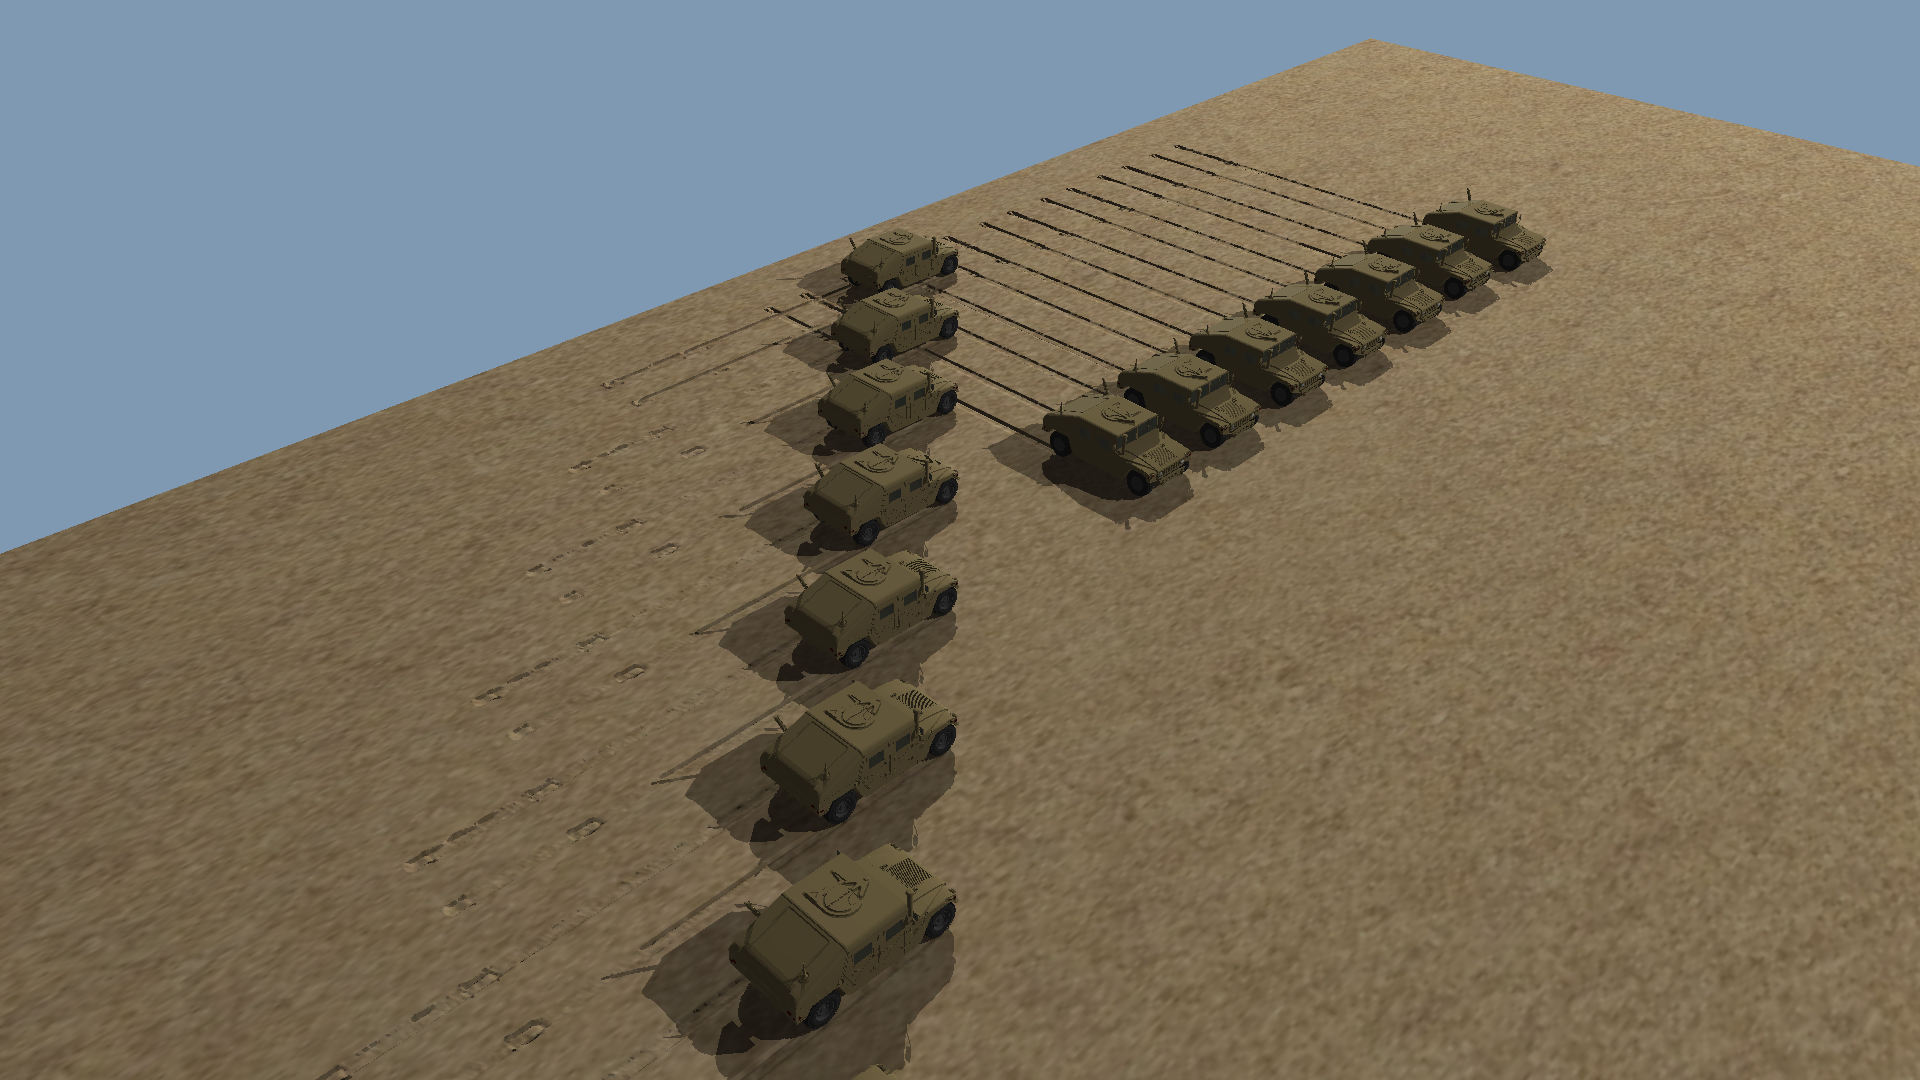
\includegraphics[width=\columnwidth]{Figs/Syn-SCM-setup.png}
    \caption{Environment used for SynChrono scaling analysis for agents operating on SCM terrain. Two lines of vehicles move across a rectangular patch, crossing orthogonally and making ruts in the SCM soil. Simulations were run on both soft and hard SCM terrain, as well as on rigid terrain.}
    \label{fig:scalingenv}
\end{figure}

The scaling metric used was the Real Time Fraction (RTF), representing the amount of wall-time required to finish a simulation divided by the amount of time simulated. Running in real-time corresponds to a factor of 1, while slower than real-time corresponds to factors larger than one. The tests were run on the Euler computing cluster at the University of Wisconsin-Madison. Each node has an eight core, Broadwell-generation Intel processor; inter-node communication is facilitated via a Gigabit Ethernet interconnect. While in practice ranks would sit on as few nodes as possible to better share data, we assigned each rank to distinct cluster nodes to focus on the communication overhead for the worst-case scenario. The scaling analysis results are presented in Fig.~\ref{fig:scmscaling}. The plot shows on the $y$-axis the $ log_{10} $ of the RTF. Thus, any dot below the horizontal $x$-axis is associated with an experiment that ran faster than real time. Simulations on the rigid terrain ran with an RTF of 0.2 and simulations on either type of SCM terrain (hard or soft) ran with an RTF of approximately 80. The RTF value of 80 is independent of the of SCM soil parameters (i.e. soft vs. hard), but is highly dependent on the processor performance, compiler, and compilation optimization. These results confirm weak scaling behavior: no significant performance penalty is observed for including additional agents in the simulation, even when each MPI rank is assigned to a different compute node. 

\begin{figure}
    \centering
    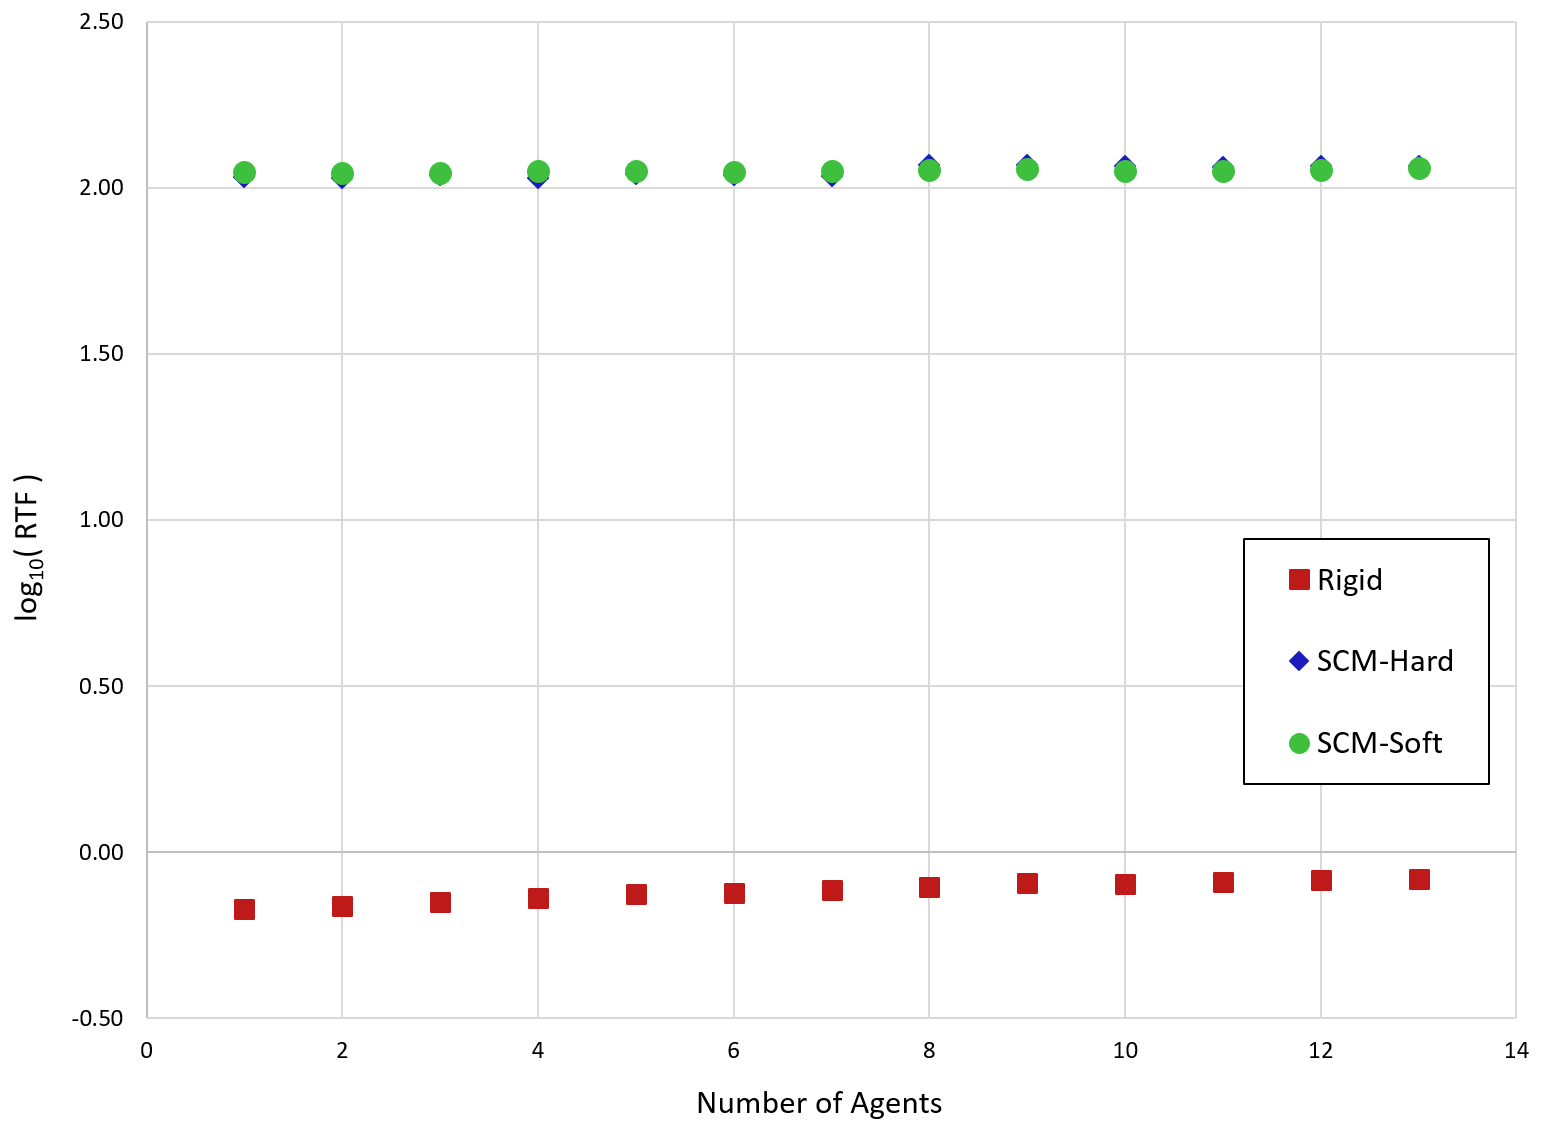
\includegraphics[width=\columnwidth]{Figs/syn_SCM_scaling.png}
    \caption{\synchrono{} scaling analysis for rigid, SCM hard, and SCM soft terrains. Logarithmic scale used.}   
    \label{fig:scmscaling}
\end{figure}

%%\FloatBarrier

%%%%%%%%%%%%%%%%%%%%%%%%%%%%%%%%%%%%%%%%%%%%%%%%%%%%%%%%%%%%%%%%%%%%%%%%%%%%%%%%%%%%%%%%%%%%%%%% 
%%%%%%%%%%%%%%%%%%%%%%%%%%%%%%  LEARNING EXAMPLE  %%%%%%%%%%%%%%%%%%%%%%%%%%%%%%%%%%%%%%%%%%%%%% 
%%%%%%%%%%%%%%%%%%%%%%%%%%%%%%%%%%%%%%%%%%%%%%%%%%%%%%%%%%%%%%%%%%%%%%%%%%%%%%%%%%%%%%%%%%%%%%%% 
\subsection{Learning to drive in a convoy}
\label{subsec:learningDemo}
Chrono can help with two tasks: learning a control policy, and testing a policy that was designed in Chrono or brought from outside. In this example, PyChrono and GymChrono are used to design a policy. SynChrono is subsequently used to test it. The RL-based learning is done on rigid terrain and its goal is to enable a vehicle to move as part of a convoy. To test it, the policy is deployed on vehicles that are part of a four-vehicle convoy driving on rigid of SCM deformable terrain. Up to three of the convoy vehicles use this policy while driving in a platoon. Thus, the possible scenarios are: three lead vehicles and one following vehicle (3L+1F), two lead and two followers (2L+2F), and one lead and three followers (1L+3F). The lead vehicles are programmed to follow a path defined by way-points; for all purposes, these can be considered human driven. A follower vehicle is autonomous and uses the learned policy to follow the vehicle in front of it. In doing so, it should not crash in the vehicle ahead of it, and avoid hitting obstacles in the vicinity of the path. 

\paragraph{Designing a policy.} The policy was obtained through training using a custom implementation of the PPO reinforcement learning algorithm leveraging PyTorch~\cite{paszke2017PyTorch} as the Deep Learning framework. The agent is a HMMWV vehicle modeled in Chrono::Vehicle. The goal of the training process is to develop a control policy that enables an agent (in this case the HMMWV) to drive in a convoy. For training, to increase the randomness of the path and thus the robustness of the control, two different path types were used on a 90x90 meters area. The first is S-shaped, starting from a corner and finishing in the opposite corner; the second is C-shaped, starting and finishing on the same side of the driving area. To further increase the randomness, these paths can be flipped along the $y$-axis (left-right) and rotated about the vertical $z$-axis to obtain 16 different possible paths. The starting point is picked randomly within the first half of the path as shown in Fig.~\ref{fig:paths}. Eight obstacles placed near the path are randomly selected from various rock, tree, and bush assets. 

%\todo[inline]{SB: Two options, pick your favorite.}
%\begin{figure}
%    \centering
%    \includegraphics[width=\columnwidth]{Figs/all_paths.pdf}
%    \caption{All possible paths. The dashed lines represent the segment of the path in which the simulation episode can start}   
%    \label{fig:paths_all}
%\end{figure}

\begin{figure}
    \centering
    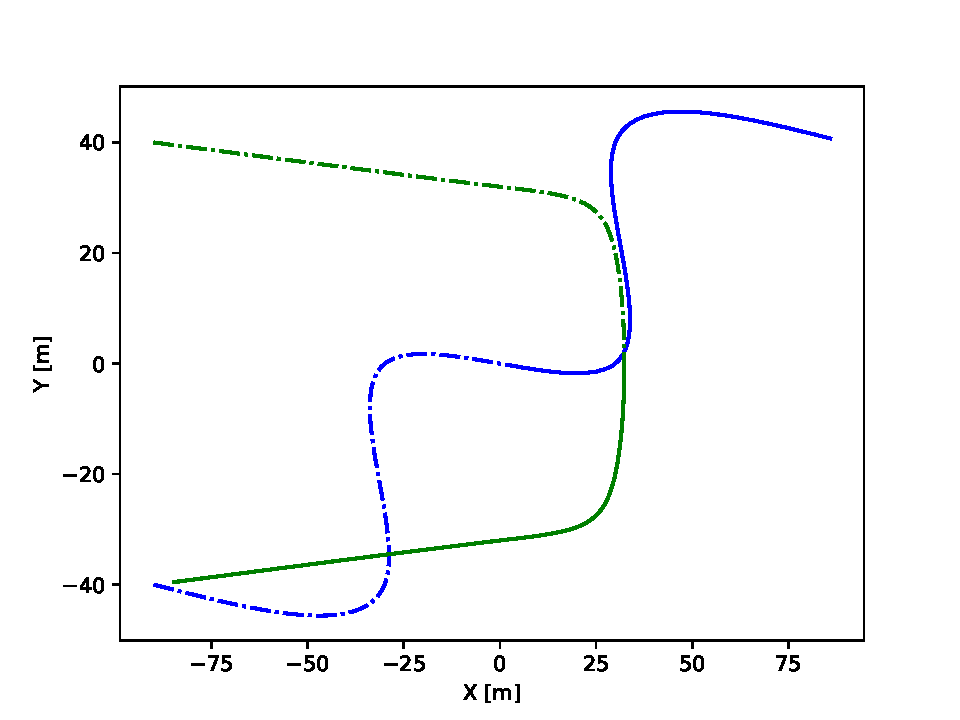
\includegraphics[width=\columnwidth]{Figs/base_paths.pdf} 
    \caption{The double S and C paths used during training. Each one of these is randomly flipped and rotated, resulting in 16 different possible paths. The dashed lines represent the segment of the path in which the simulation episode can start.}
    \label{fig:paths}
\end{figure}

In order for the agent to accomplish its task, the vehicle must be aware of its surroundings. To that end, the HMMWV used two sensors simulated in Chrono::Sensor: a GPS sensor, and an RGB camera placed on the front bumper. The camera, which updates at 30 Hz, has a resolution of 80 $\times$ 45 pixels. This level of resolution suffices, since detailed features that can be extracted from higher resolution images are not needed by the control policy. Furthermore, given that the dataset contains one image per interaction, images of too high resolution can quickly deplete the available GPU memory due to the increased memory footprint of the NN update process. As such, large images that are contained in observations are typically avoided. 

As with any other RL environment, an observation and a reward is provided to the ML algorithm at each timestep. Subsequently, the agent must perform an action prescribed by the ML algorithm in order to maximize the reward collected. The action is a 2-dimensional array: the first element is a steering value; the second is a combined throttling and braking value. The choice of collapsing throttle and brake control into the same action was taken to avoid simultaneous braking and throttling and because throttling and braking both directly control the vehicle's acceleration. 

The agent is rewarded only when it successfully stays behind the leader, meaning a reward is provided when the angle between the heading of the leader and the follower is in the range $[-\pi/4, \pi/4]$. When this condition is met, the agent receives the maximum reward if it keeps an optimal distance (within a prescribed tolerance) from the lead vehicle. In other words, the follower is rewarded when it stays in a sector of an annulus centered at the leader. When the vehicle is outside the desired area, the reward decreases hyperbolically. 
\begin{figure*}
    \centering
    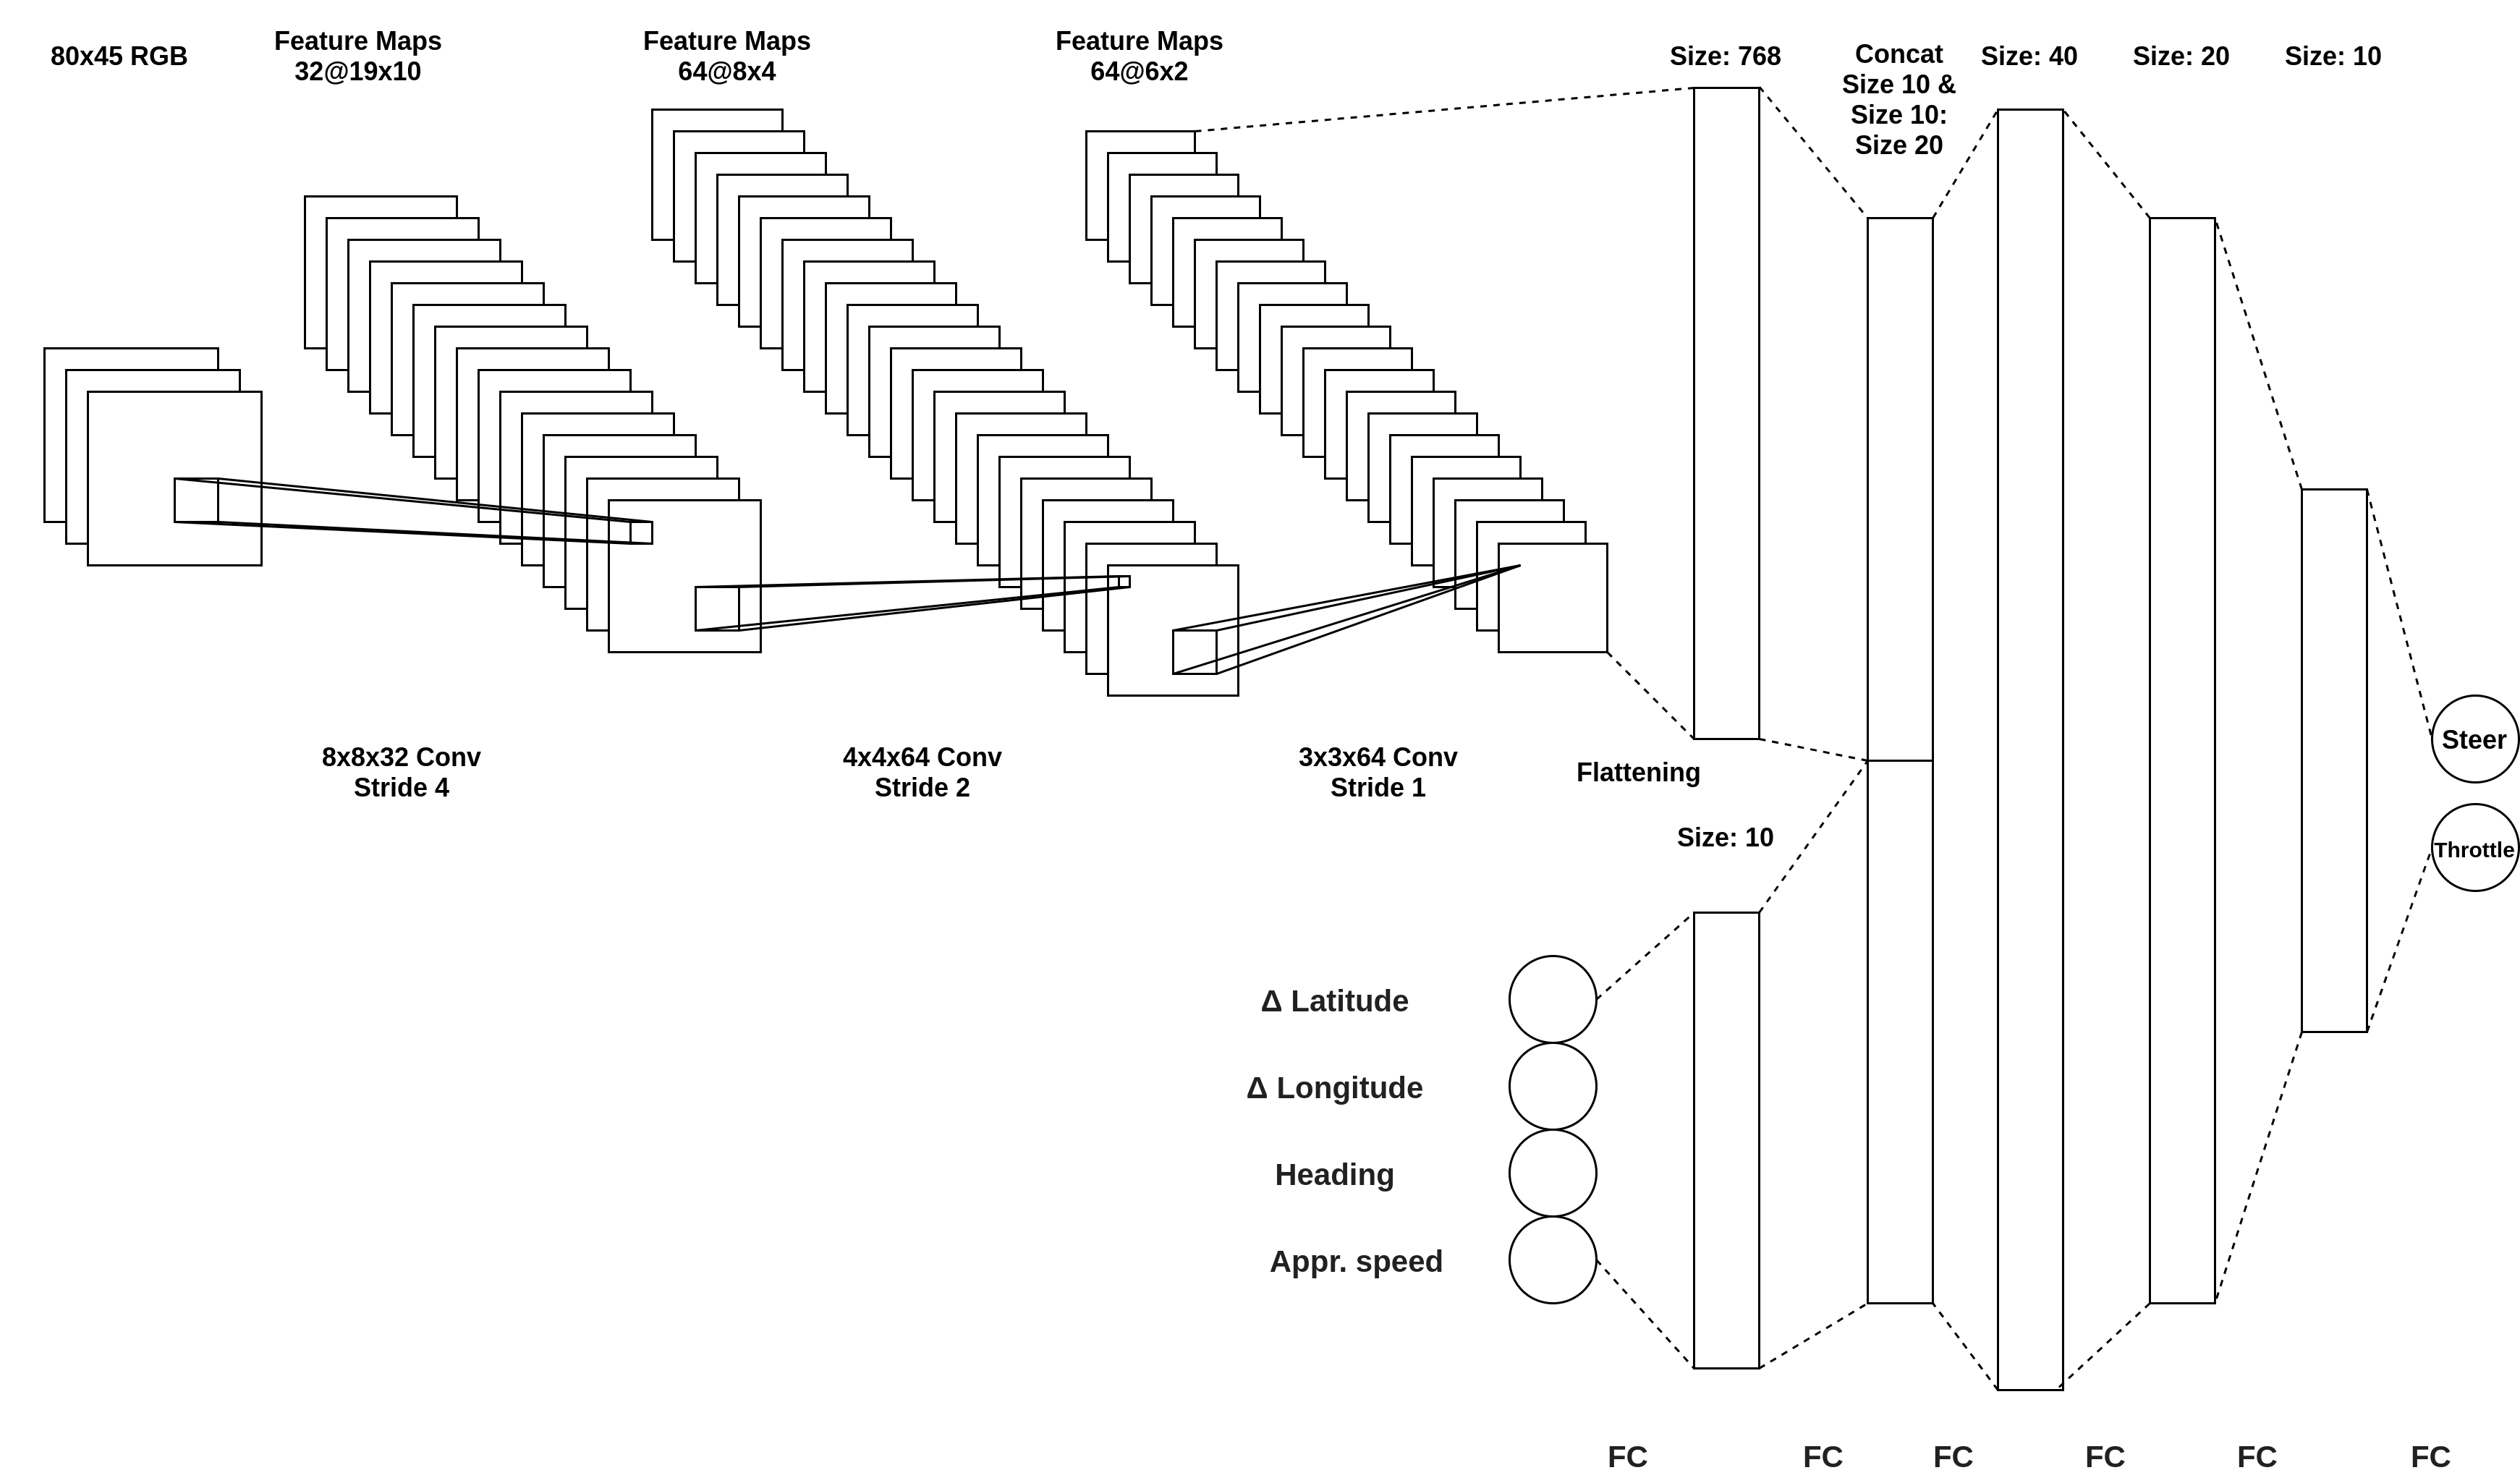
\includegraphics[angle=90,width=0.6\linewidth]{Figs/MS_NN.png}
    \caption{{\small Sensor Fusion NN architecture.}}   
    \label{fig:NNarch}
\end{figure*}

The learning draws on information from several sensors, whose output is organized into two tuples. The first element is a 80 $\times$ 45 $\times$ 3 RGB image. The second is a vector of four values: the latitude and longitude difference between the leader and the follower; the heading according to the compass; and the speed at which the follower is approaching the leader. This multi-sensor observation required the NN architecture to incorporate an input composed of a 3D and a 1D tensor. The image is processed in a Convolutional Neural Network (CNN) as in~\cite{Mnih13}. Its output is then concatenated with the output of the one Fully Connected (FC) hidden layer Deep Neural Network (DNN) which takes the 1D Tensor as input. Their concatenated output is then processed by three FC hidden layers. The architecture of the model is shown in Fig.~\ref{fig:NNarch}.

RL-based training requires a very large number of iterations. Three decisions helped speed up the learning process: ($i$) the lead vehicles were not simulated, but only rendered at the correct location and orientation (as this has no bearing for sensing purposes); ($ii$) a reduced-order model of the HMMWV vehicle was used in the first stage of training, with the more computationally demanding full vehicle model substituted during the training process (see Fig.~\ref{fig:Rewards}) to further refine the NN parameters; and ($iii$) the learning process was accelerated using the OpenAI~\cite{Brockman16Gym} Baselines tool for environment parallelization, thus allowing several simulations running simultaneously to speed up the collection of the dataset samples.

%{\SBELcomment{NOTE: In the caption for Fig.~\ref{fig:Rewards} we talk about things that we don't touch upon in the text. Caption is hard to understand (except switching to full vehicle -- we do touch on this in the text).}} {\SBELcomment{SB: I got rid of some unnecessary details}}

\begin{figure}
	\centering
	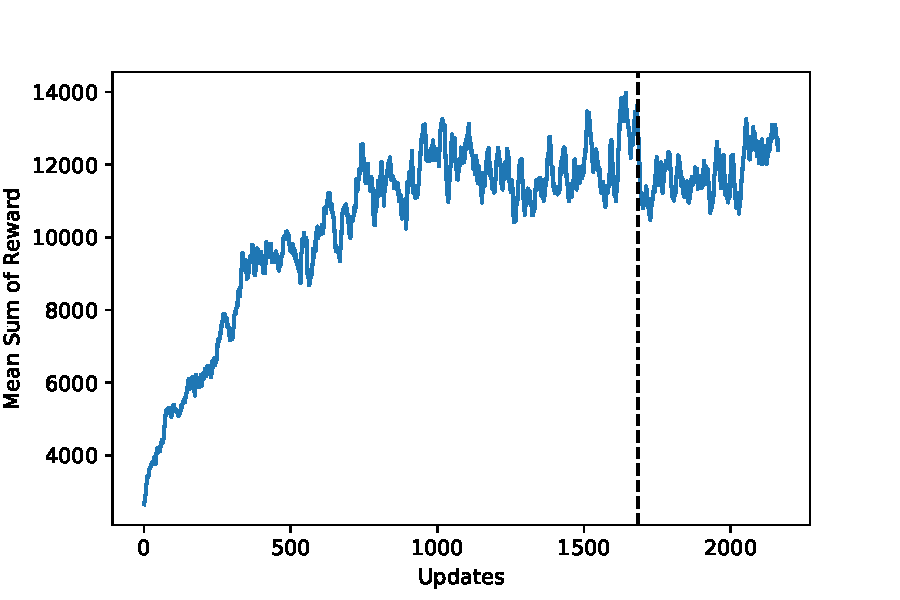
\includegraphics[width=\columnwidth]{Figs/rewards.pdf}
	\caption{Plot of the moving average of the sum of collected rewards with respect to the policy updates (updated every 1500 interactions). The vertical dashed line represents the switch from the reduced to the full HMMWV model.}
	\label{fig:Rewards}
\end{figure}


\paragraph{Testing of learned policy.}  The AA control policy derived in PyChrono and GymChrono was tested in SynChrono for various convoy setups while operating on three terrain types. The platoons were 3L+1F, 2L+2F, and 1L+3F. The terrains were rigid, SCM hard (silt-like), and SCM soft (snow-like). This leads to a set of nine \textit{platooning scenarios} in which the AA policy was tested. 

\begin{figure*}
    \centering
    \begin{subfigure}{0.33\textwidth}
        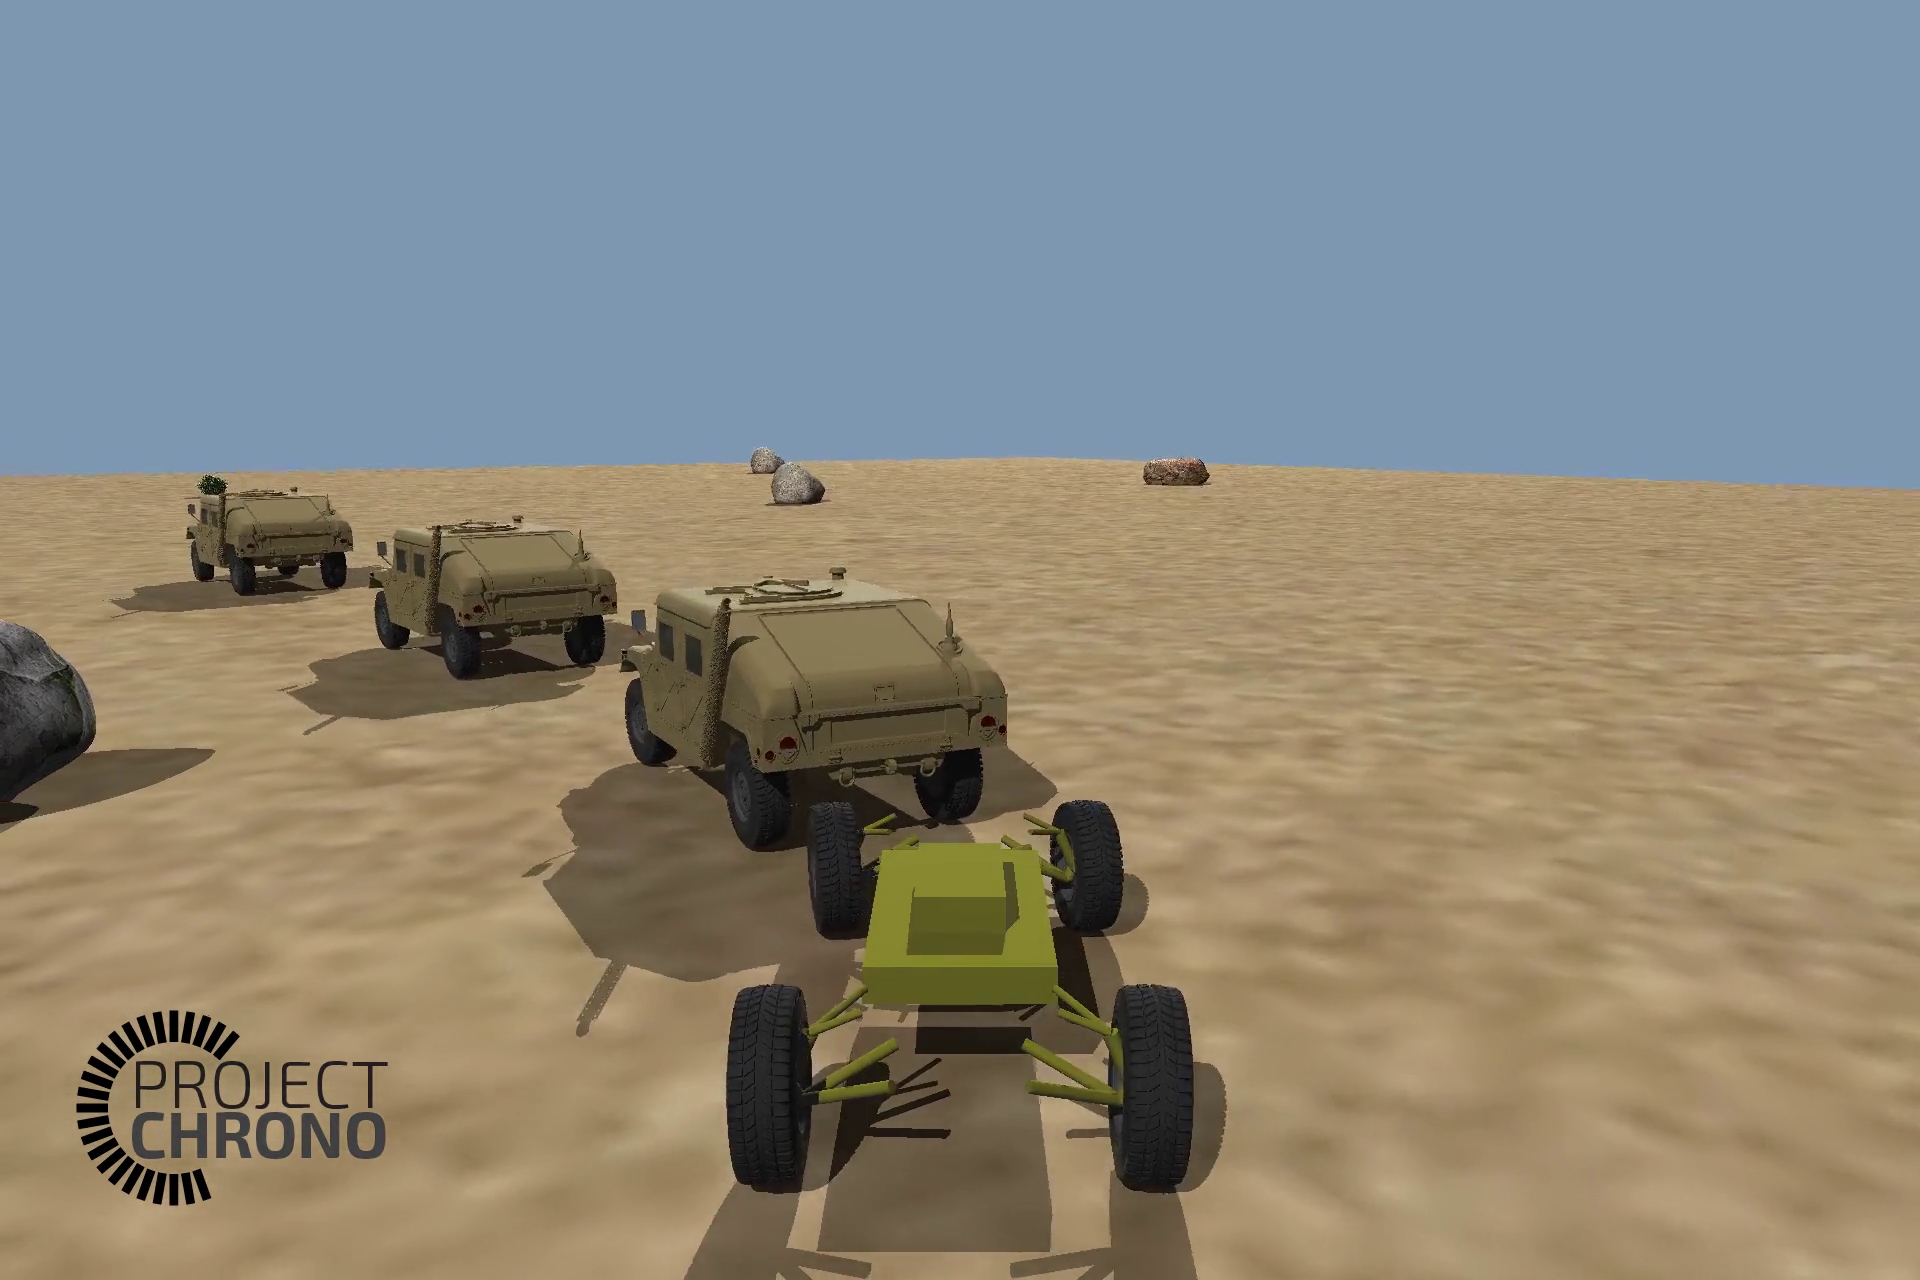
\includegraphics[width=\linewidth]{Figs/Demonstration/rigid_1i_3f.png}
        \caption{} \label{fig:rigid13}
    \end{subfigure}%
    \begin{subfigure}{0.33\textwidth}
        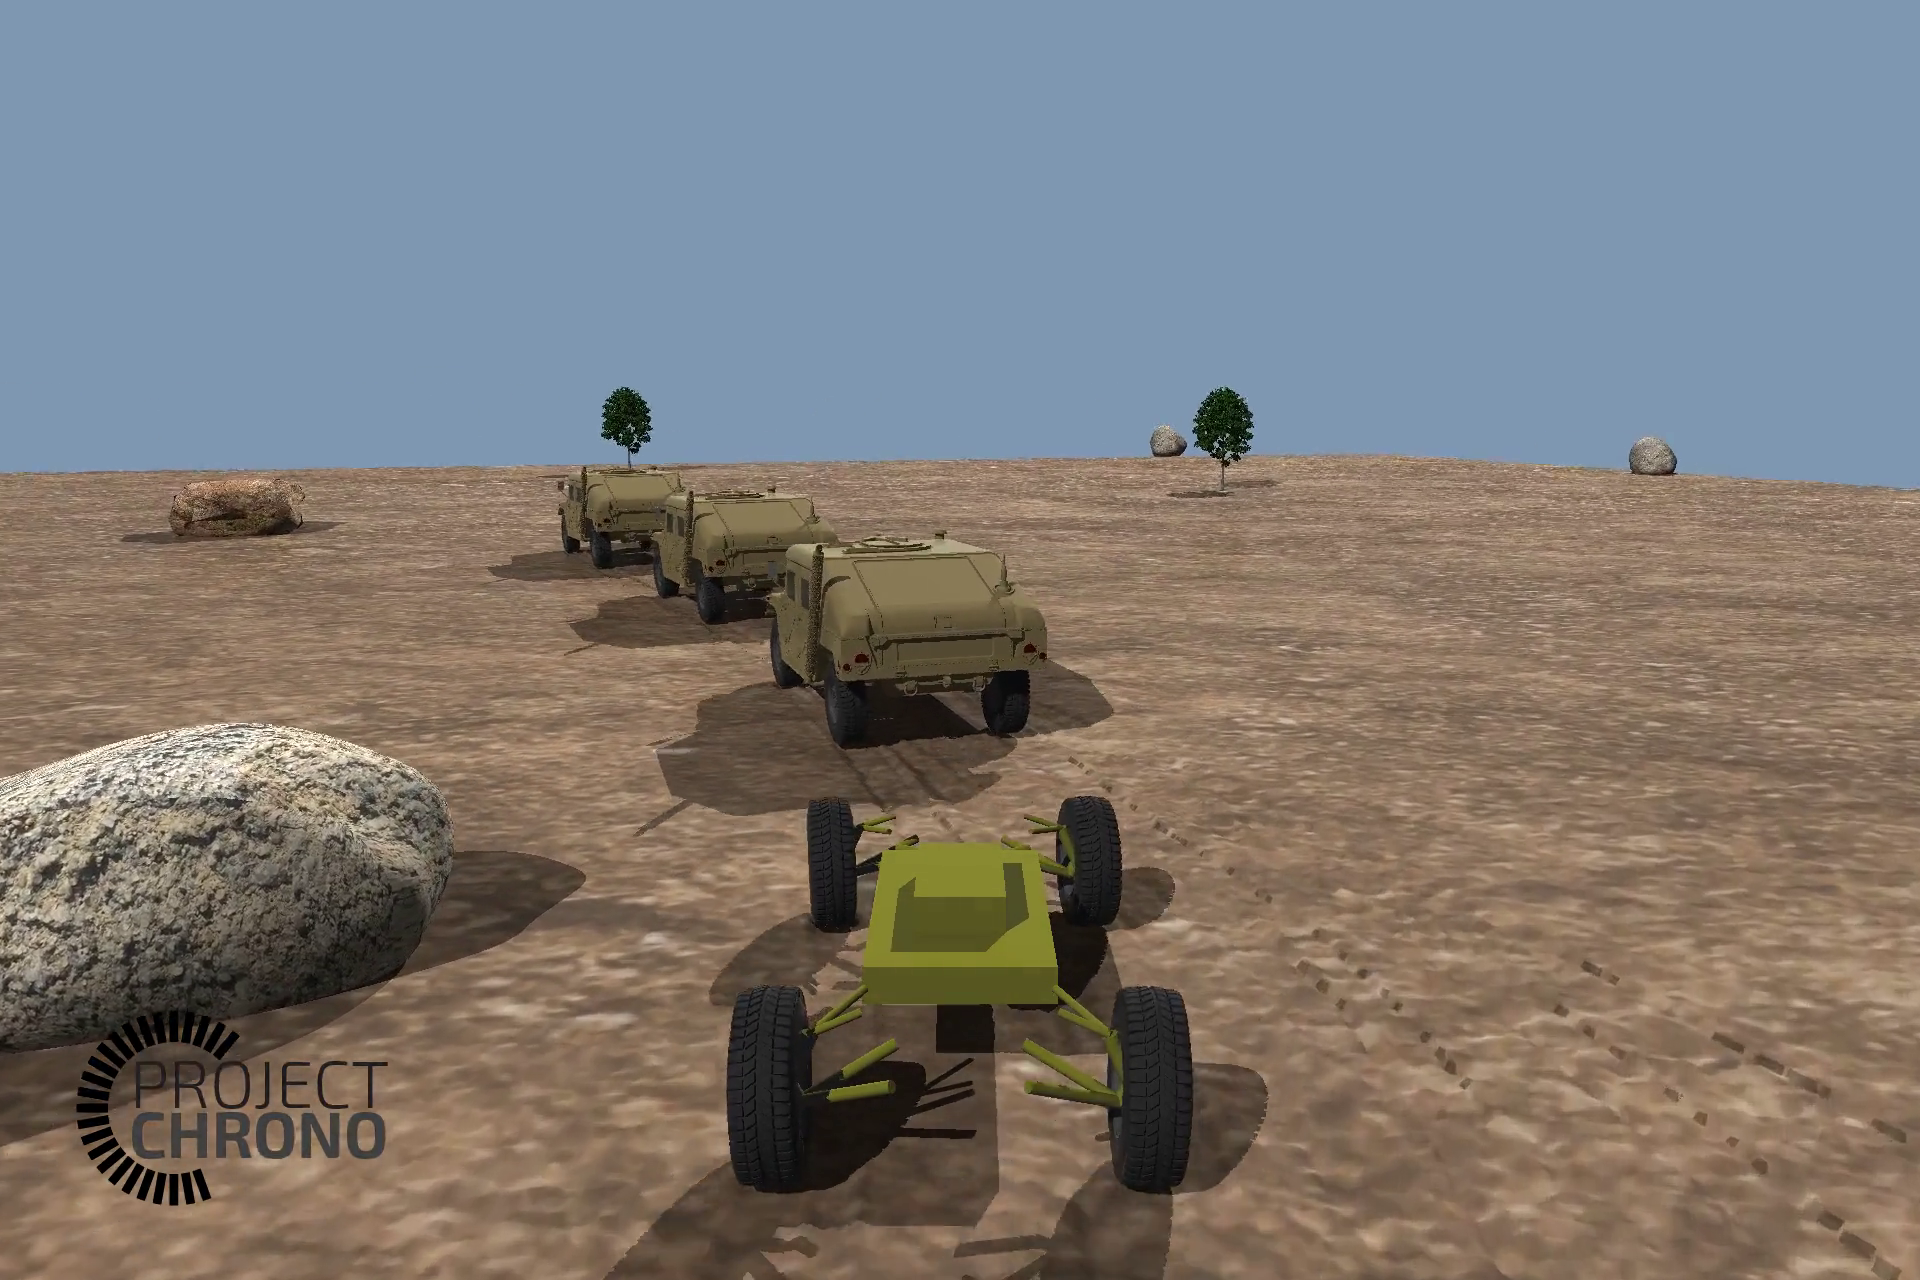
\includegraphics[width=\linewidth]{Figs/Demonstration/hard_1i_3f.png}
        \caption{} \label{fig:hard13}
    \end{subfigure}%
    \begin{subfigure}{0.33\textwidth}
        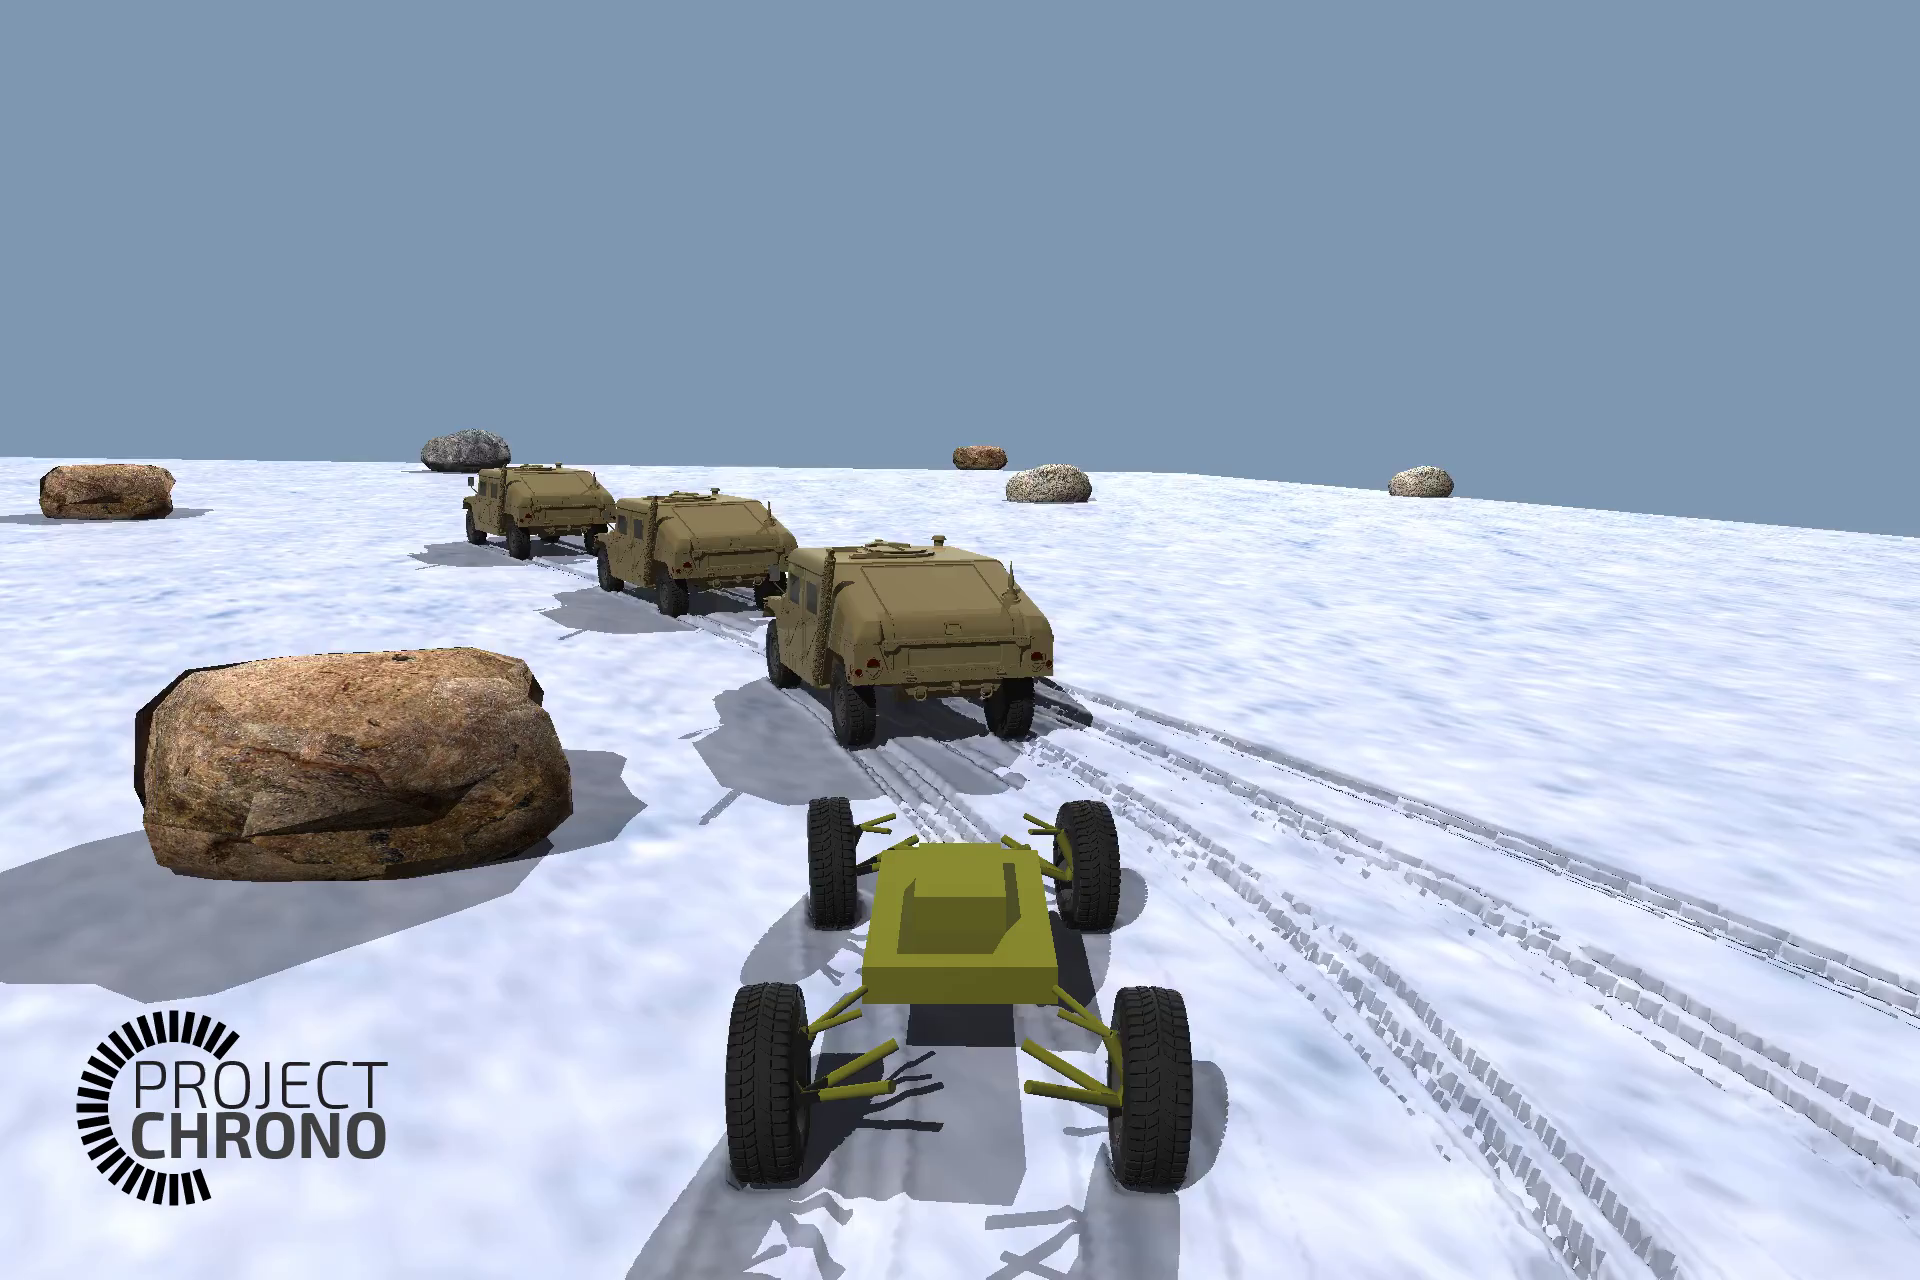
\includegraphics[width=\linewidth]{Figs/Demonstration/soft_1i_3f.png}
        \caption{} \label{fig:soft13}
    \end{subfigure}%
    \caption{Still frames from attached third person camera: (a) rigid terrain; (b) hard SCM terrain; (c) soft SCM terrain.}   
    \label{fig:simscreenshots}
\end{figure*}


For each platooning scenario, data recorded to evaluate the performance of the convoy included position, velocity, and acceleration for each of the four vehicles. In addition, a high definition camera sensor was attached to the last vehicle in the convoy in order to visualize the simulation. Still frames captured with this camera are shown in Fig.~\ref{fig:simscreenshots}. Full length videos of these experiments are available online \cite{simsPaperGVSETS2020}. Different ground textures were used to further differentiate between the three terrain types. Dirt, mud and snow textures were each used for the rigid, hard SCM and soft SCM terrains, respectively. In Table~\ref{tab:vehiclepositions}, top-down views of the convoy trajectories are shown for each platooning scenario. Each leader is represented as a solid line and each follower is seen as a dashed line.

\begin{table*}
    \centering
    \caption{2D Positions of each vehicle in each simulation configuration}
    \label{tab:vehiclepositions}
    \begin{tabular} { cccc }
         & \hspace*{.75cm}3L$ + $1F& \hspace*{.75cm}2L$ + $2F& \hspace*{.75cm}1L$ + $3F \\
        %\hline 
        %\\ 
        {\rotatebox[origin=c]{90}{Rigid Terrain}}&
        \parbox[c]{2.02in}{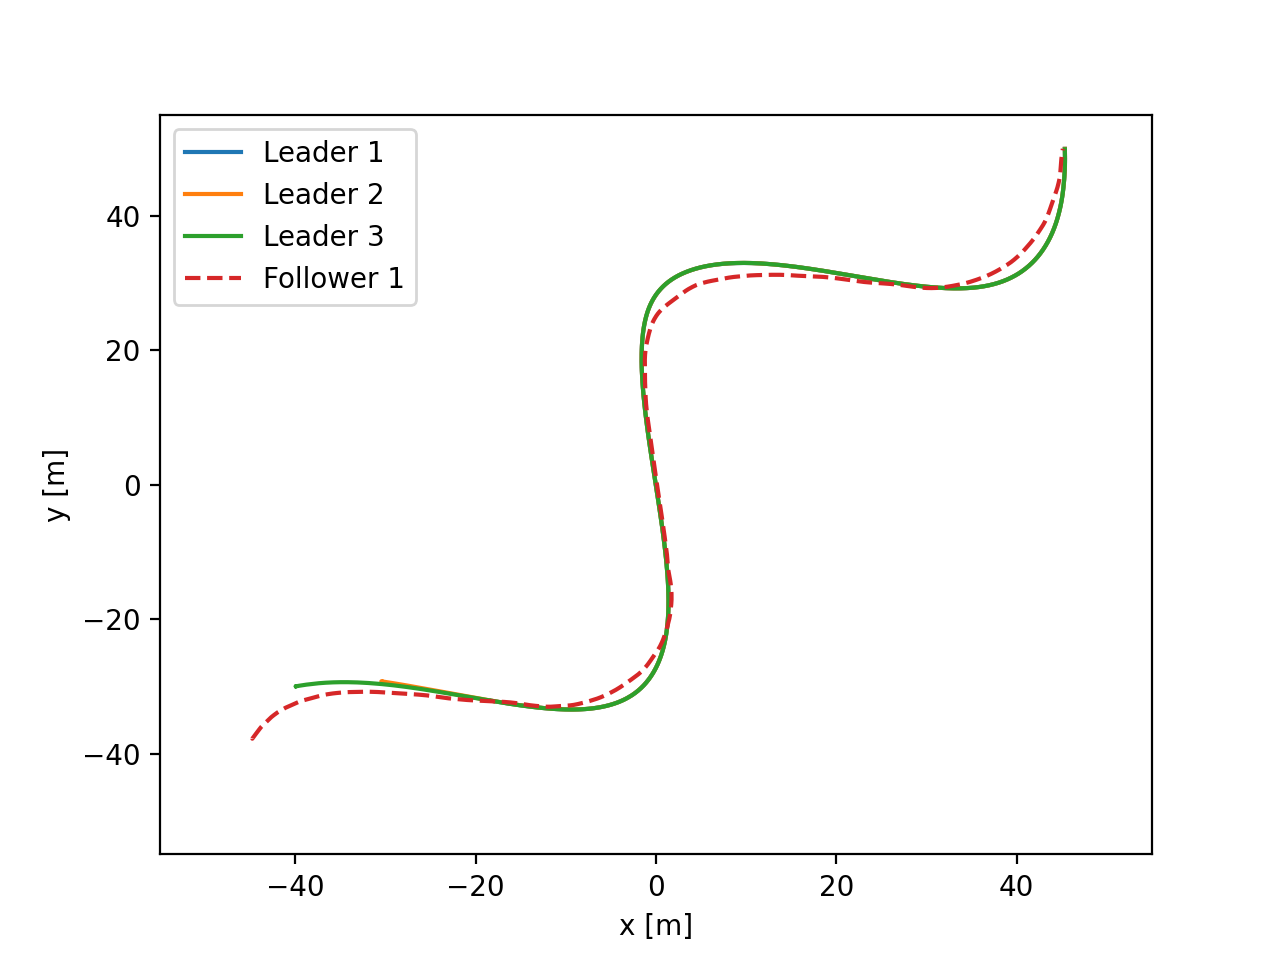
\includegraphics[height=1.8in]{Figs/Demonstration/3f_1i_rigid_positions.png}}&
        \parbox[c]{2.02in}{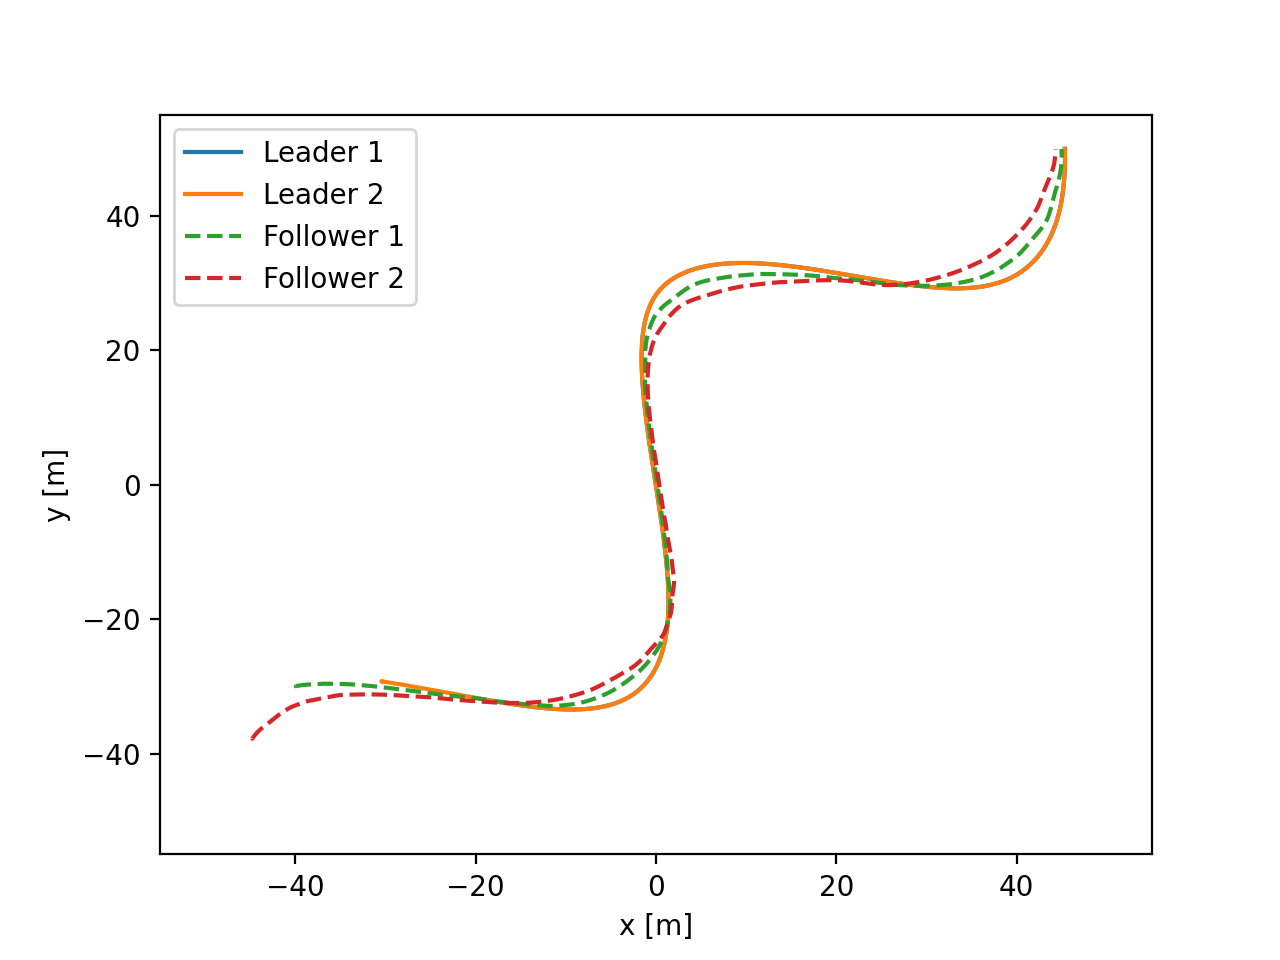
\includegraphics[height=1.8in]{Figs/Demonstration/2f_2i_rigid_positions.png}}&
        \parbox[c]{2.02in}{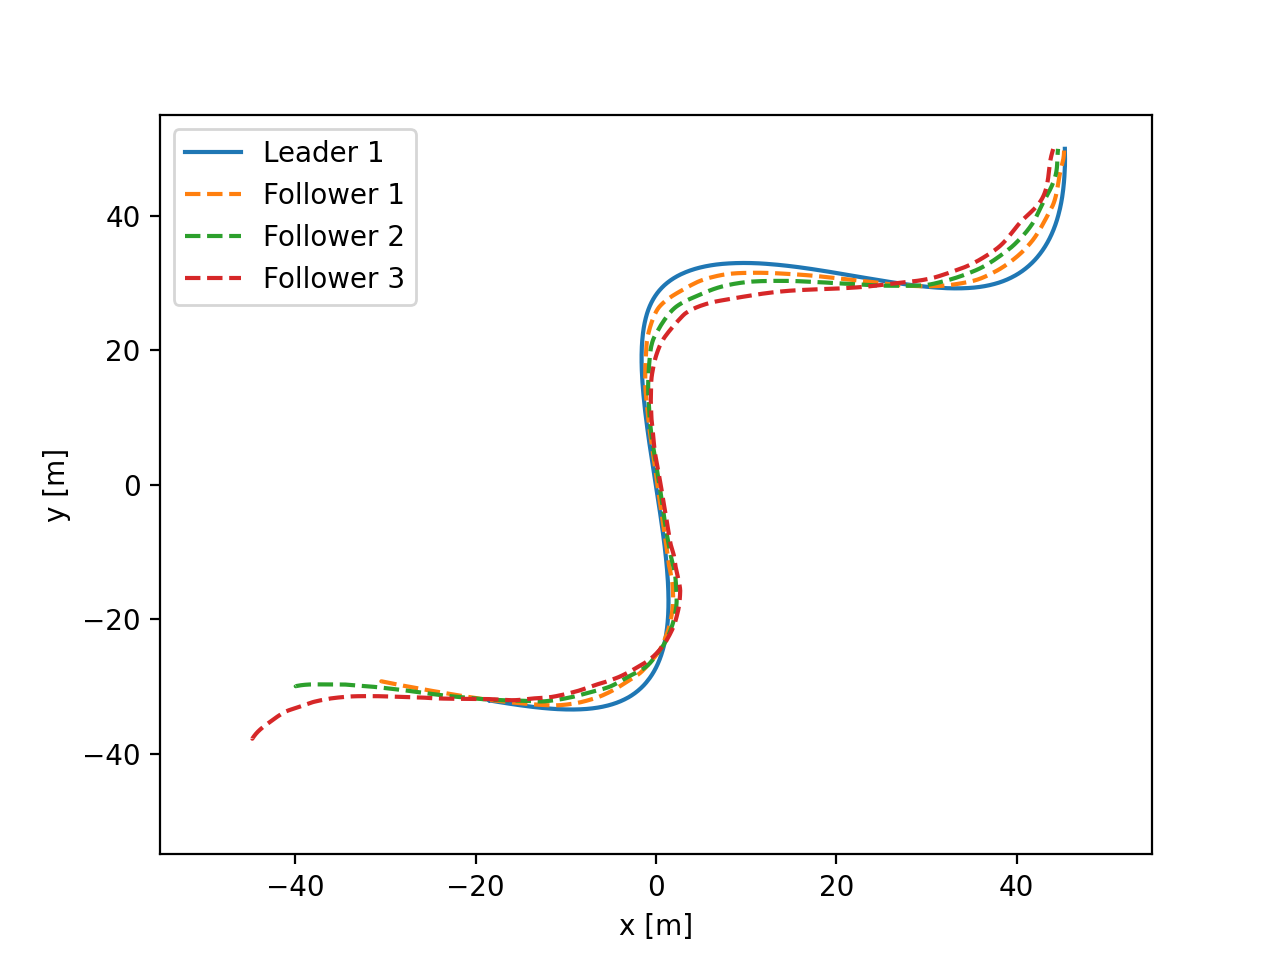
\includegraphics[height=1.8in]{Figs/Demonstration/1f_3i_rigid_positions.png}}\\
        %\newline \\
        %\hline 
        %\\ 
        {\rotatebox[origin=c]{90}{Hard SCM}}&
        \parbox[c]{2.02in}{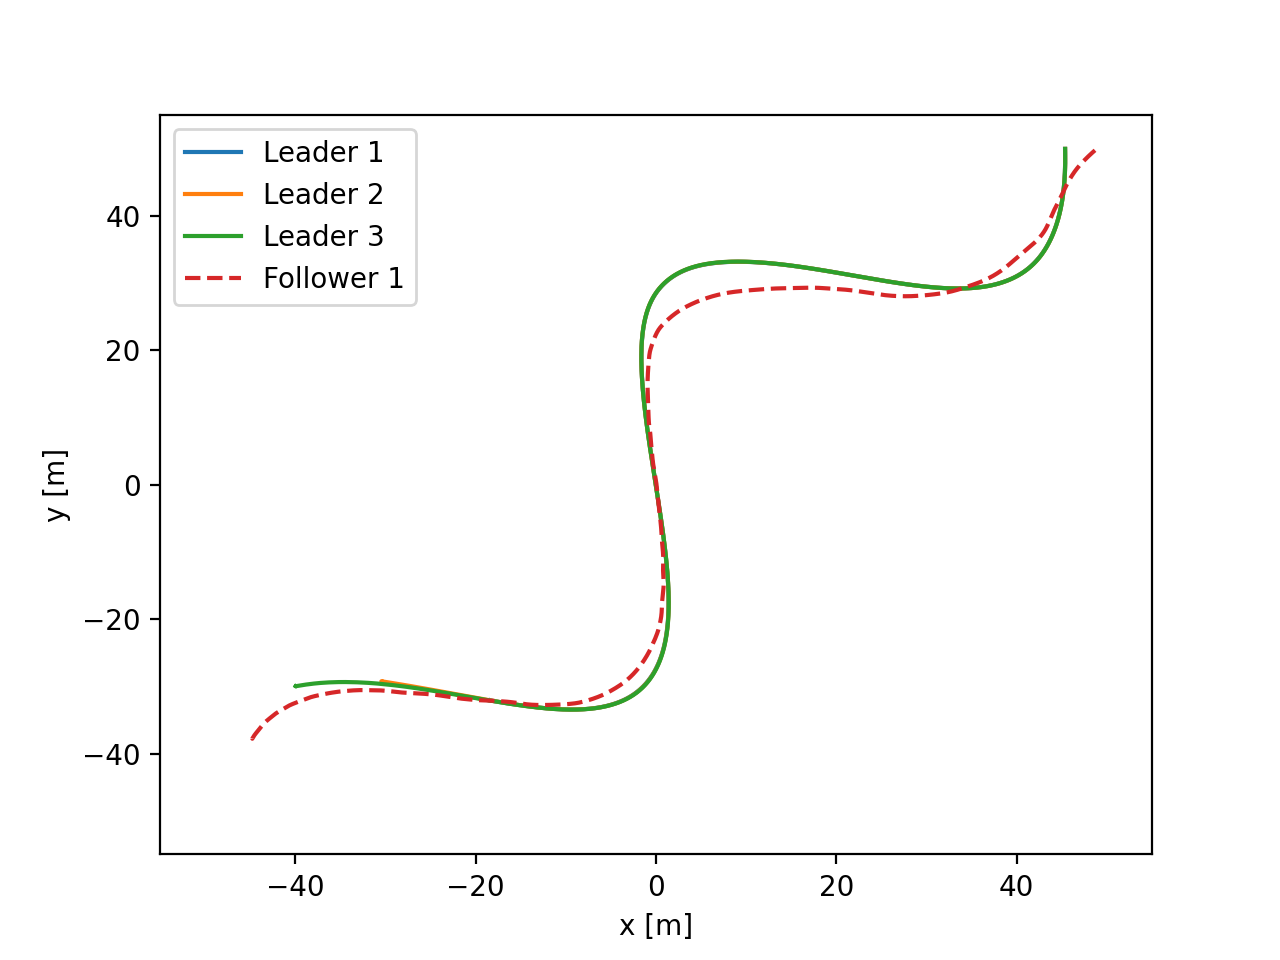
\includegraphics[height=1.8in]{Figs/Demonstration/3f_1i_hard_positions.png}}&
        \parbox[c]{2.02in}{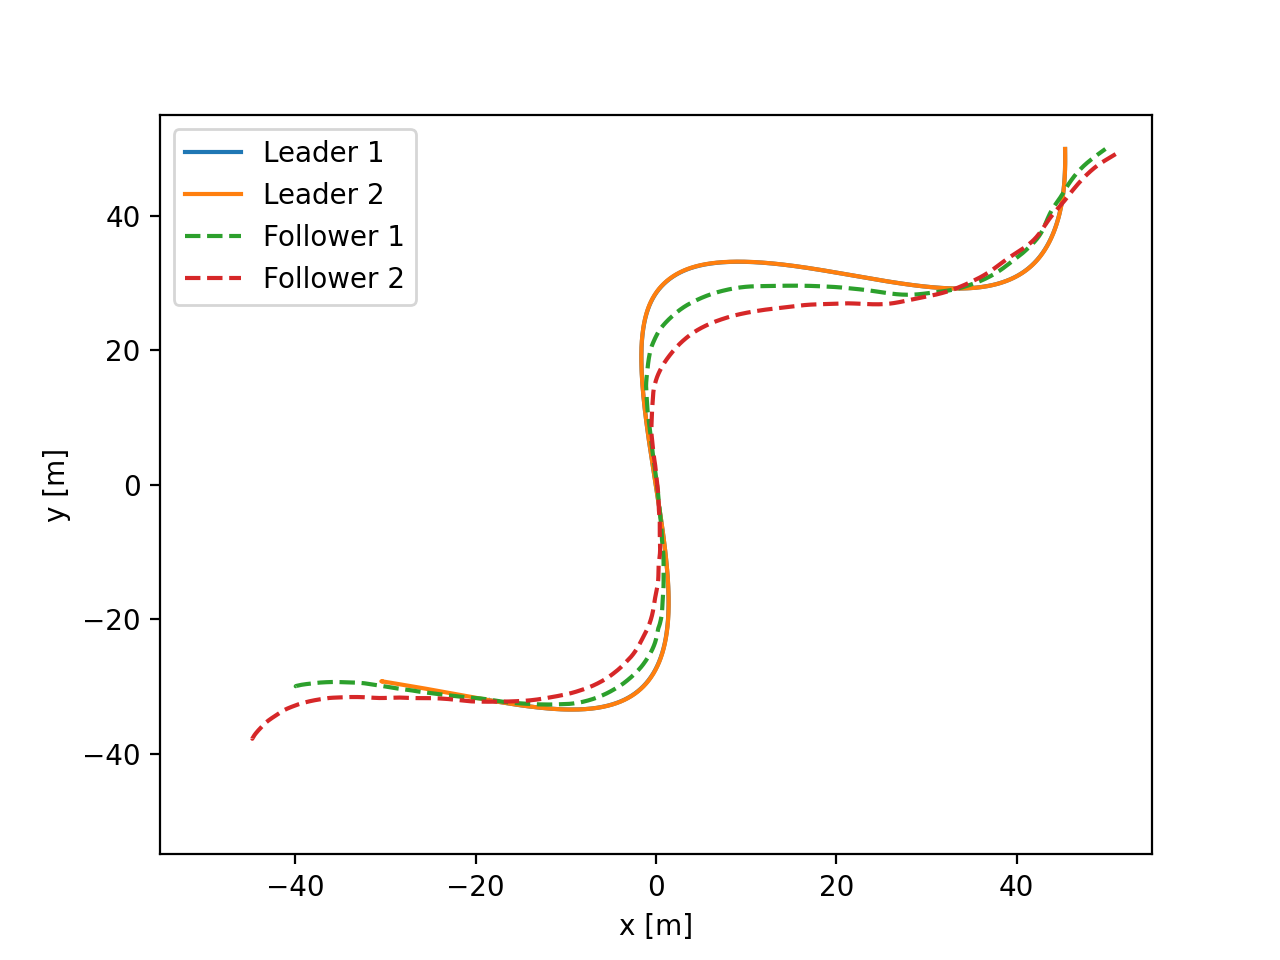
\includegraphics[height=1.8in]{Figs/Demonstration/2f_2i_hard_positions.png}}&
        \parbox[c]{2.02in}{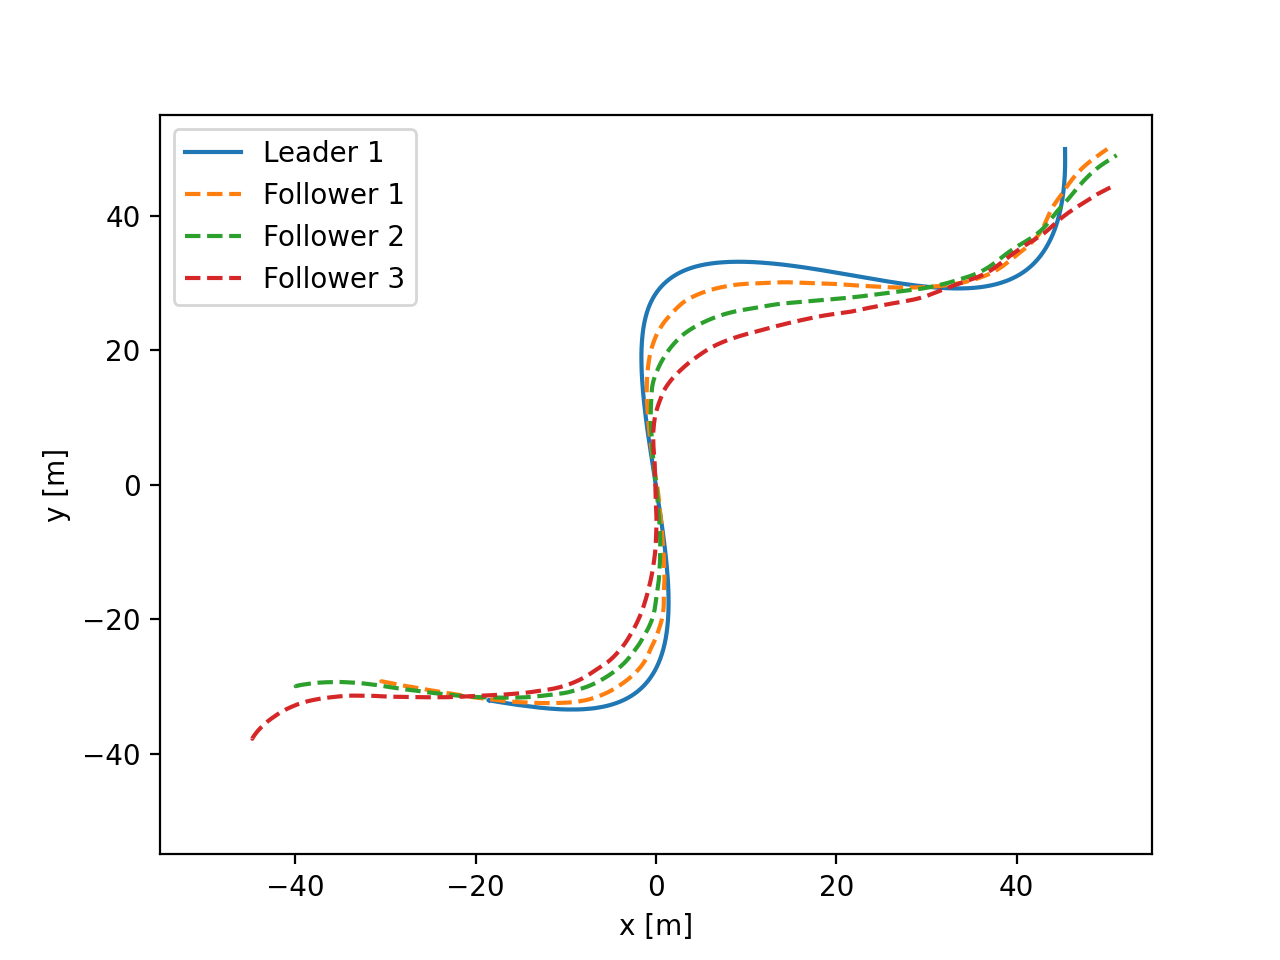
\includegraphics[height=1.8in]{Figs/Demonstration/1f_3i_hard_positions.png}}\\
        %\newline \\
        %\hline 
        %\\
        {\rotatebox[origin=c]{90}{Soft SCM}}&
        \parbox[c]{2.02in}{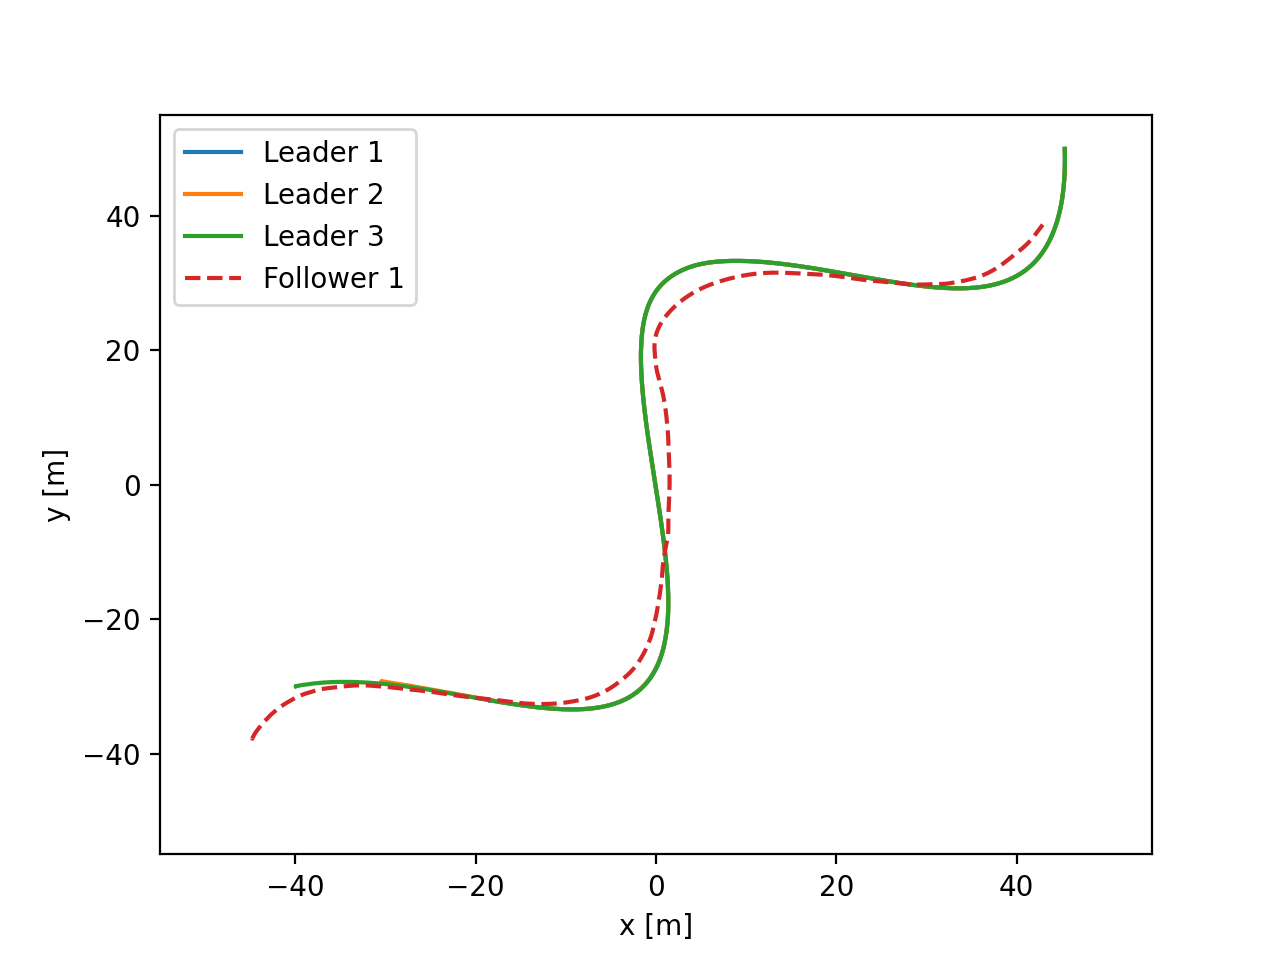
\includegraphics[height=1.8in]{Figs/Demonstration/3f_1i_soft_positions.png}}&
        \parbox[c]{2.02in}{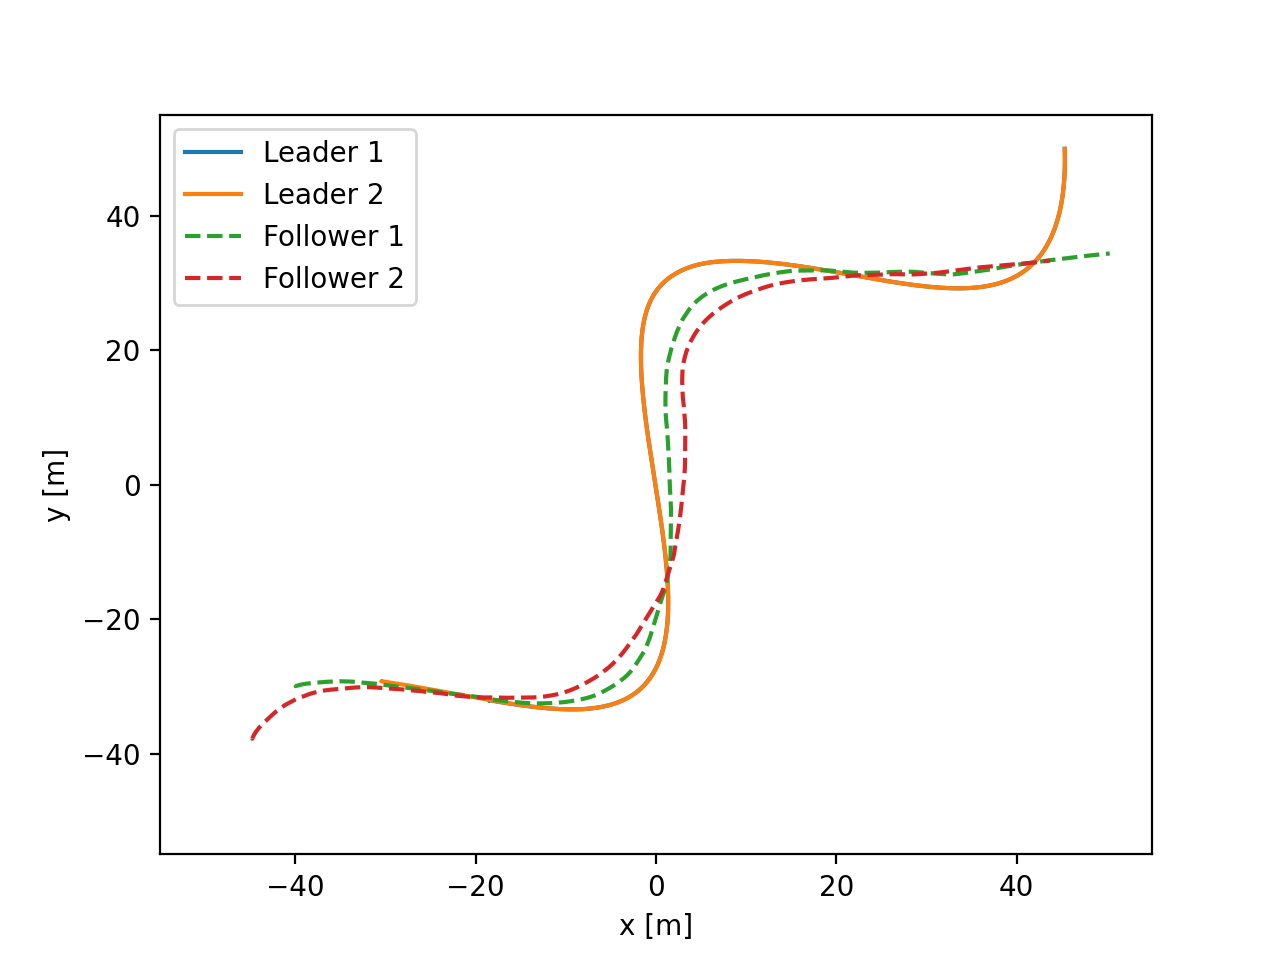
\includegraphics[height=1.8in]{Figs/Demonstration/2f_2i_soft_positions.png}}&
        \parbox[c]{2.02in}{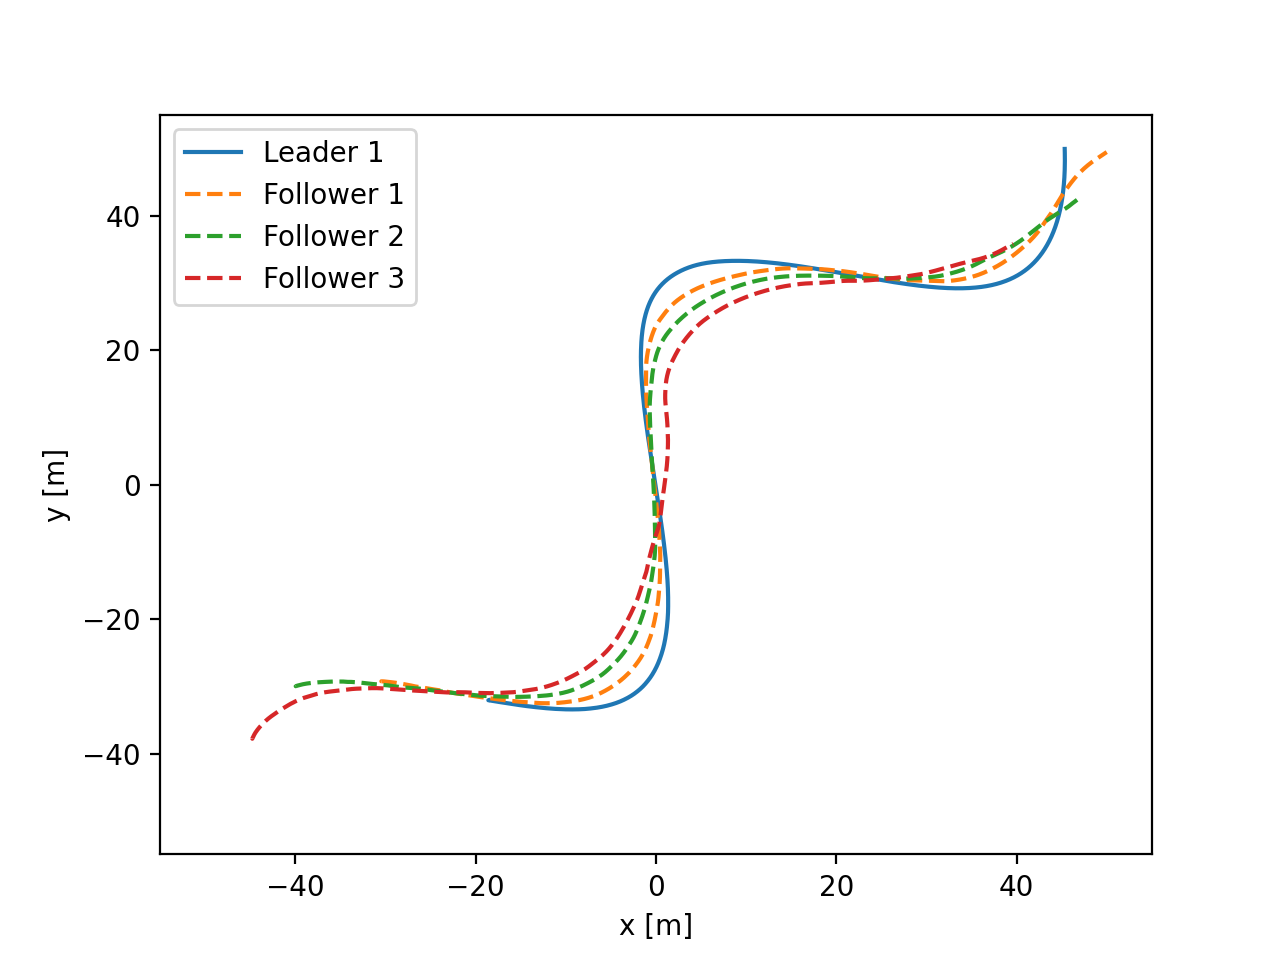
\includegraphics[height=1.8in]{Figs/Demonstration/1f_3i_soft_positions.png}}
        %\newline \\ 
        %\hline \\
    \end{tabular}
\end{table*}

As seen in Table~\ref{tab:vehiclepositions}, each simulation configuration resulted in a different reaction of the follower vehicles. As indicated in \S\ref{subsec:learningDemo}, the training process rewards the follower for being within a certain angle \emph{and} distance of the leader. As a result, this provided some room for the vehicle to deviate from the prescribed path. This can be seen clearly in the three leader vehicle configuration, where the follower diverges from its leaders' path at a small margin. In the 2L+2F and 1L+3F platooning scenarios, this effect is magnified, as for each additional follower, a similar effect is observed; hence, the last follower in the one leader configuration tests is approximately three times further from the prescribed path around corners compared to the 3L+1F configuration. On occasion, this artifact led to the last vehicle clipping obstacles positioned on the inside of these corners, which points to a weakness of the control policy design.

\begin{figure}
	\centering
	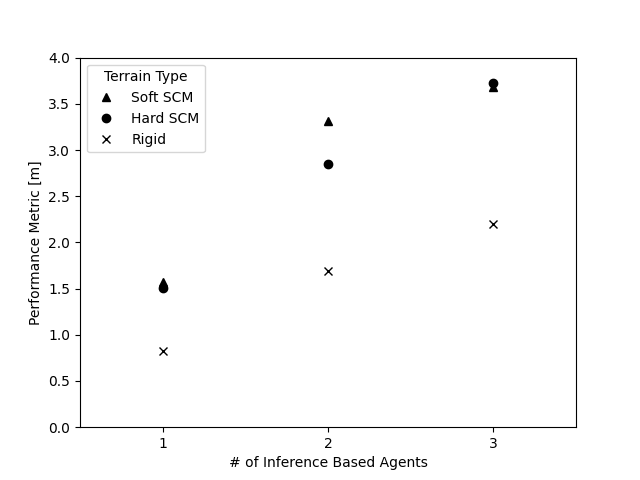
\includegraphics[width=1\columnwidth]{Figs/Demonstration/error_vs_agent.png}
	\caption{{\small Performance metric vs. the number of leader vehicles. The performance metric is the integrated error between the leader's and follower's paths divided by the length of the leader's path.}} 
	\label{fig:errorvsagent}
\end{figure}
As the terrain becomes softer, the followers tend to deviate more from the leader's path. This trend is noticeable in the images of Table~\ref{tab:vehiclepositions}. We quantified the drift by calculating a performance metric defined as the area between the paths of the leader vehicle and of the last following vehicle in the convoy divided by the length of the leader's path. A value of zero would indicate a perfect convoy maneuver in which followers run in the tracks of the lead vehicle. The results presented in Fig.~\ref{fig:errorvsagent} indicate that the convoy is best maintained on rigid terrain and when the platoon contains a single follower. As expected, the worst performance under this metric is observed in snow-like conditions for a platoon with three followers.

\begin{figure}
    \centering
    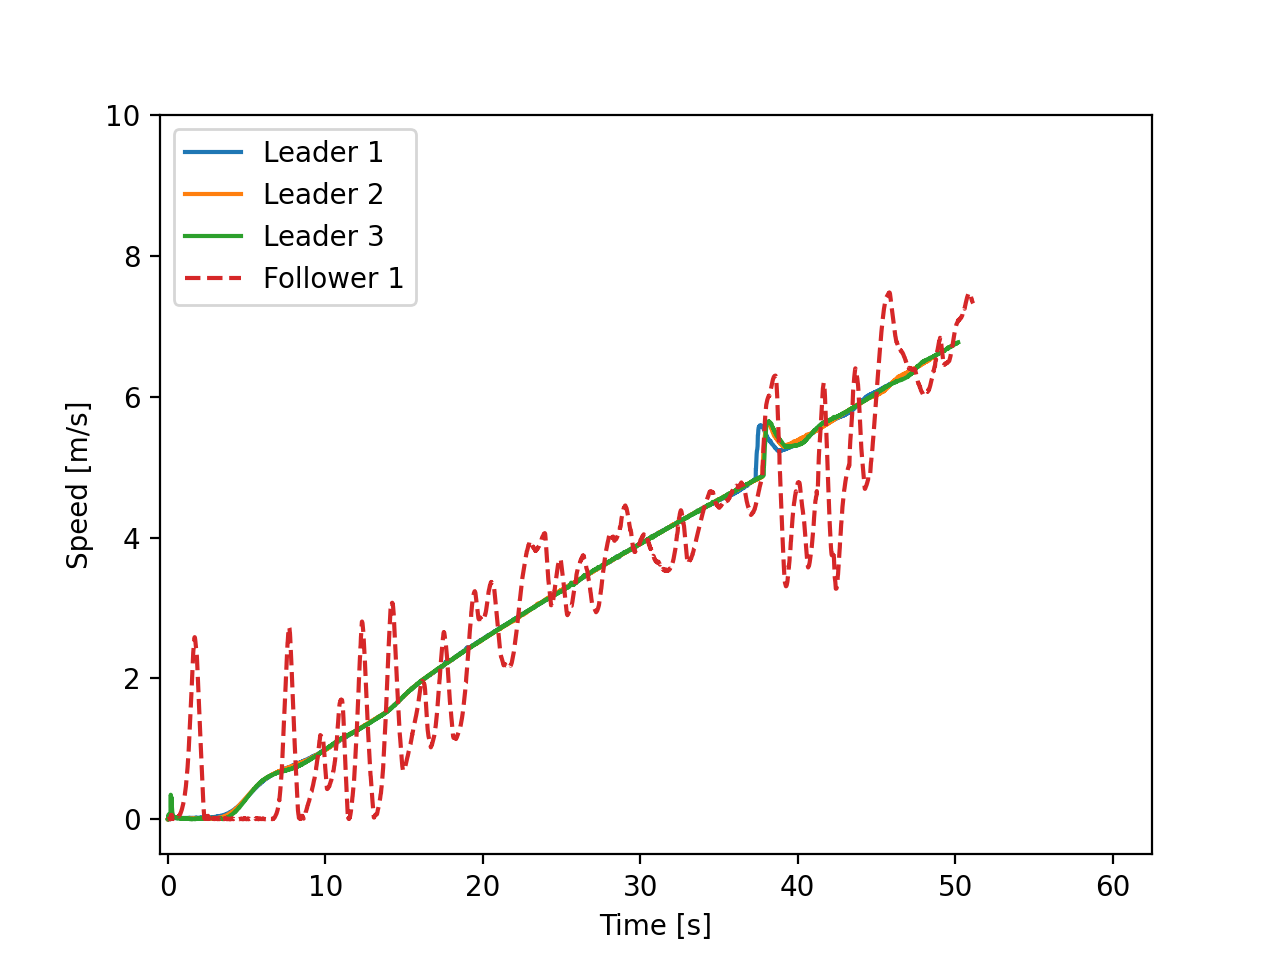
\includegraphics[width=\columnwidth]{Figs/Demonstration/3f_1i_rigid_velocities.png}
    \caption{{\small Speed of each vehicle in the 3L$ + $1F configuration; rigid terrain.}}
    \label{fig:rigid31vel}
\end{figure}
%
\begin{figure}
    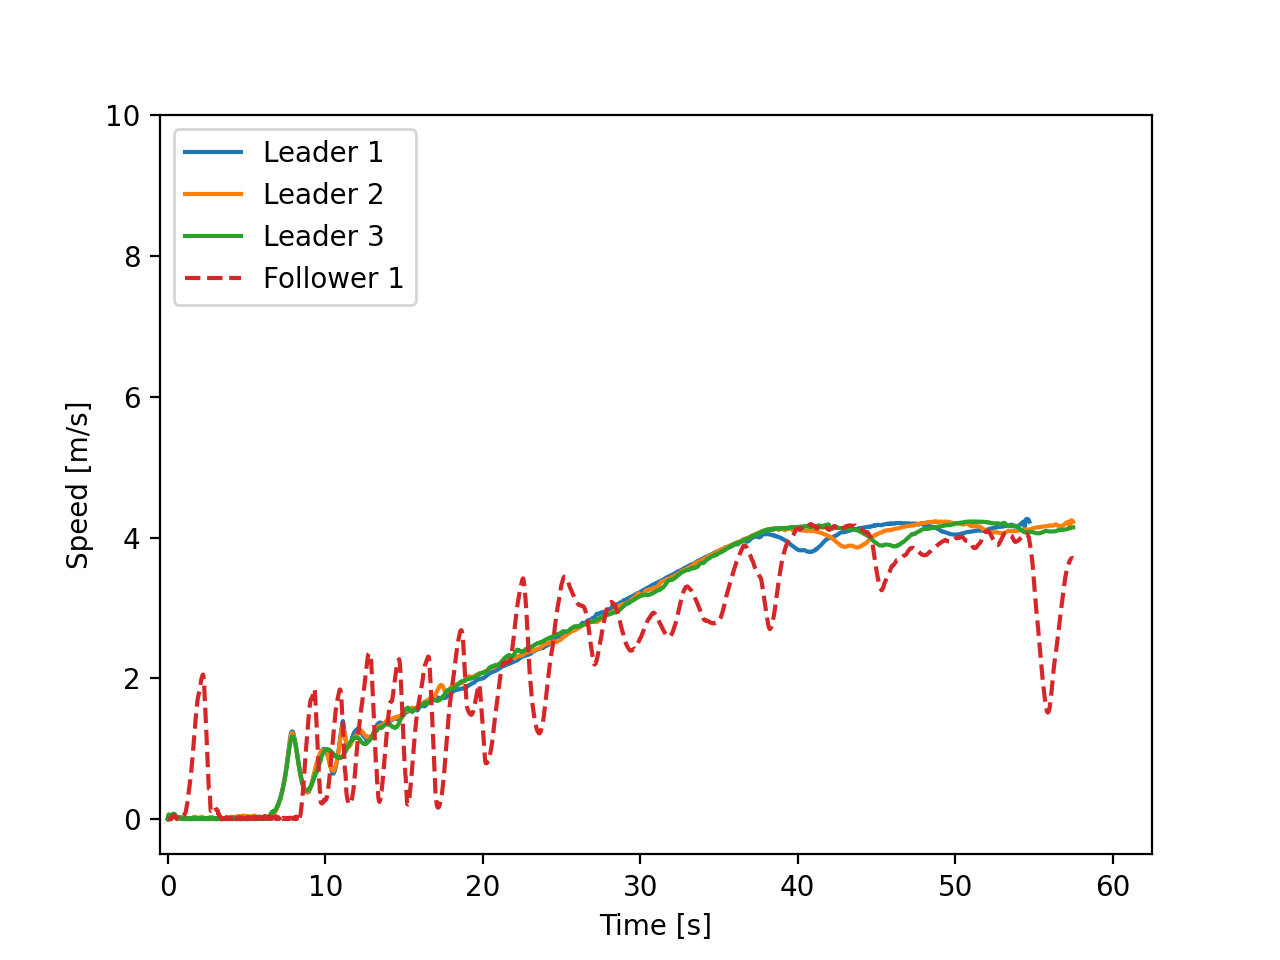
\includegraphics[width=\columnwidth]{Figs/Demonstration/3f_1i_soft_velocities.png}
    \caption{{\small Speed of each vehicle in the 3L$ + $1F configuration; soft SCM terrain.}}
    \label{fig:soft31vel} 
\end{figure}
For each simulation test, the leader vehicles utilize PID-based lateral and longitudinal controllers to follow the predetermined path with a prescribed target speed (with the latter linearly increasing in time). The speed profiles of the four vehicles in the 3L+1F configuration on rigid and soft SCM terrain are presented in Figs.~\ref{fig:rigid31vel} and \ref{fig:soft31vel}, respectively.  In these simulations, the three leader vehicles use identical parameters for their path-following and adaptive cruise-control PID controllers.  While the speed of the leader vehicles can increase continuously throughout the simulation length when driven over rigid terrain, due to the increased motion resistance on the soft SCM soil the speed levels off approximately 40 seconds into the simulation.

As seen in these plots, the speed profiles of the follower vehicles are not smooth; even though they generally follow the same overall rate of increase as that prescribed for the leader vehicles, their motion is jerky with successive acceleration and braking.  This can also be seen in the associated videos \cite{simsPaperGVSETS2020}.  Improvements to the RL-based policy to mitigate this behavior are currently being pursued and will be included in the final version of the manuscript.

%\FloatBarrier

%% ============================================================ 
%% ============================================================ 
\section{CONCLUSIONS. FUTURE WORK}\label{s:conclusion}
This contribution discussed a Chrono-centric simulation platform designed to facilitate the design and testing of control policies for AAs operating in off-road conditions. This simulation platform targets deployment on computing clusters and displays weak scaling. The platform draws on a physics-based simulation engine, has templates for wheeled and tracked vehicles, enforces space and time coherence, allows for human-in-the-loop scenarios, provides sensor simulation capabilities, has a bridge to ROS, can simulate mobility on fully resolved, continuum, or SCM representations of the terrain, and is open source. This software framework is used here to design an RL-based control policy that allows an AA to drive in a convoy formation. Once the learning is completed, one, two, or three AAs were deployed in a four-vehicle convoy that drove on paths different from those used in training. The learning took place on rigid terrain but was demonstrated to work when deployed on AAs that operate on deformable SCM soils. The virtual environments used in testing differed in textures and colors from the ones used in the training, thus demonstrating robustness of the inferred policy which relies on inputs from an RGB camera sensor. Unsurprisingly, the fewer AAs in the platoon, the tighter it managed to follow a prescribed path. The final version of the paper will augment the present work in two respects: it will contain a statistical analysis that quantifies the effectiveness of the RL-derived control policy and will discuss an improved RL-based policy that smooths out the driving style of the AAs, which is currently jerky.


%% ============================================================

\section*{Acknowledgments}
The Euler supercomputer used in this work contains hardware procured through the Army Research Office DURIP instrumentation grant W911NF1810476. Support for terramechanics research is provided through US Army Research Office project W911NF1910431. Ongoing support for core {\chrono} development is provided by National Science Foundation project CISE1835674. Ongoing support for SynChrono development is provided by National Science Foundation project CPS1739869. Support for the development of \chronomod{Vehicle} was provided by U.S. Army GVSC grant W56HZV-08-C-0236. Support for the development of \chronomod{Sensor} and {\synchrono} has been provided by the SAFER-SIM program, which is funded through a grant from the U.S. Department of Transportation's University Transportation Centers Program (69A3551747131).



%% ============================================================
\bibliographystyle{unsrt}
\bibliography{Bib/refsAutonomousVehicles,Bib/refsMachineLearning,Bib/refsChronoSpecific,Bib/refsCompSci,Bib/refsDEM,Bib/refsFSI,Bib/refsGraphics,Bib/refsMBS,Bib/refsRobotics,Bib/refsSBELspecific,Bib/refsSensors,Bib/refsTerramech,Bib/refsDRL}


%% ============================================================
%%% ============================================================

\clearpage
From this point on is old stuff
\section{FRAMEWORK}\label{s:framework}

%% ============================================================

\subsection{\chronomod{Sensor}}\label{s:ChSensor}

\chrono{} and \synchrono{} and \chronomod{Vehicle} \chronomod{Sensor} is a Project \chrono{} submodule for sensing simulation. Supported sensors include camera, lidar, \gps{}, and \imu{}. Exteroceptive sensing (camera, \lidar{}) leverages headless, off-screen ray-tracing support via \optix{}. \chronomod{Sensor} seeks to generate realistic data that is equivalent to data from its physical counterpart. To this end, \chronomod{Sensor} supports modeling and simulation of the noise and distortion observed on the data streams of physical sensors. Examples of \chronomod{Sensor} used to simulate a scaled autonomous vehicle navigating a closed course are shown below.

\begin{figure}
	\centering
	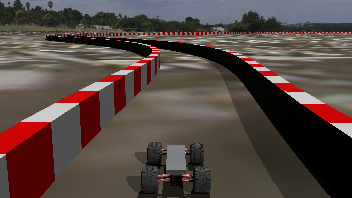
\includegraphics[width=0.8\columnwidth]{Figs/AV-third-person.png}
	\caption{{\small Third person perspective of scaled autonomous vehicle navigating a course using a simulated camera and \lidar{}.}}   
	\label{fig:avthirdperson}
\end{figure}

\begin{figure}
	\centering
	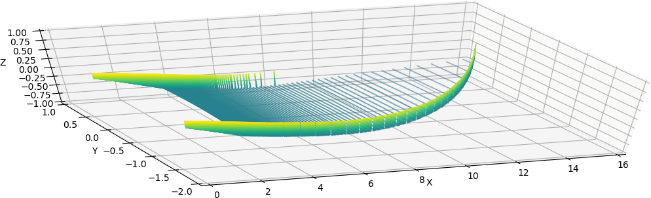
\includegraphics[width=0.8\columnwidth]{Figs/AV-lidar.png}
	\caption{{\small Lidar data showing the course from the perspective of the virtual vehicle. The data is used in the control stack to detect the barriers and determine the desired path.}}   
	\label{fig:avlidar}
\end{figure}

\begin{figure}
	\centering
	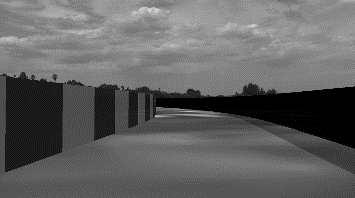
\includegraphics[width=0.8\columnwidth]{Figs/AV-greyscale.png}
	\caption{{\small Image from a simulated grayscale camera mounted to the front of the scaled autonomous vehicle.}}   
	\label{fig:avgreyscale}
\end{figure}

%%============================================================

\subsection{\pychrono{} and \gymchrono{}}\label{s:pyandgym}

\pychrono{} is a package that provides Python bindings for the \chrono{} \api{}. Using an interface compiler (SWIG), the vast majority of the \chrono{} \api{} (multibody dynamics, Vehicle, Sensor, \fea{}, etc.) can be directly accessed from Python. Beyond ease of use, the Python wrapping allows interfacing \chrono{} and ML frameworks for training neural networks. \gymchrono{} provides a set of Robotics and Autonomous Driving environments leveraging \chrono{} for physics simulation and OpenAI gym support for Reinforcement Learning baselines and tools for scalable training.

%%============================================================

\subsection{\synchrono{}}\label{s:synchrono}

\synchrono{} is a software component built on top of \chrono{} that allows for a distributed-memory execution of simulation scenarios that include tens of agents. It builds off the Message Passing Interface (\mpi{}), which allows the toolset to have multiple instances of \chrono{} run simultaneously on a supercomputer/cluster/multi-core setup to allow for the distributed simulation of multiple agents (robots, tracked vehicles, wheeled vehicles, etc.) The paradigm embraced is that of running one \chrono{} agent simulation as one \mpi{} rank, with multiple ranks, say N, communicating through messages to maintain a space and time coherent solution for the N agents participating in the study. This multi-agent form of simulation distribution is possible because of the largely decoupled nature of mobility scenarios. Each agent runs in its own rank and interfaces with its dedicated control stack for software-in-the-loop control. The control stack is fed synthetic data generated by \chronomod{Sensor} and acts upon the environment through \chronomod{Vehicle} control input (throttle, steering, braking, etc.) This “one agent-to-one \chrono{} system” mapping ensures scalability over a monolithic \chrono{} system as shown in the center picture below. The control algorithm or “brain” for each agent is also configurable and can vary from complex algorithms that collect a variety of sensor data, to controls based on empirical models, to human-driven control in scenarios that are simple enough to allow real-time simulation.

\begin{figure}
	\centering
	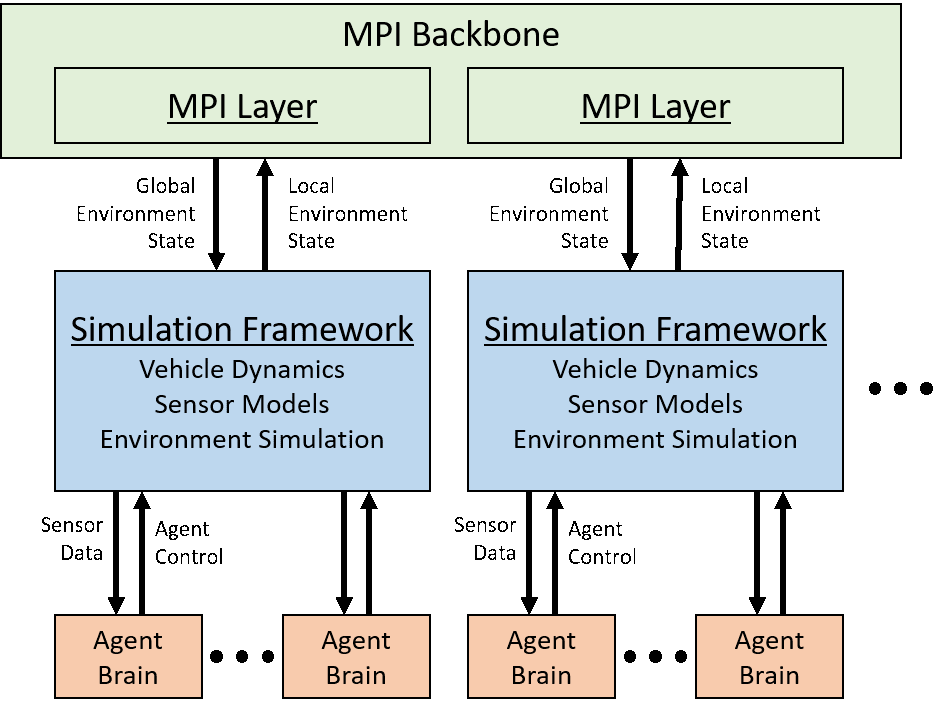
\includegraphics[width=0.8\columnwidth]{Figs/MPI-schematic.png}
	\caption{{\small Schematic of the \synchrono{} framework. Decisions are passed to the \chrono{} system for dynamics simulation and the outcome of the dynamics simulation is synchronized between ranks using \mpi{}.}}   
	\label{fig:mpischematicold}
\end{figure}

\begin{figure}
	\centering
	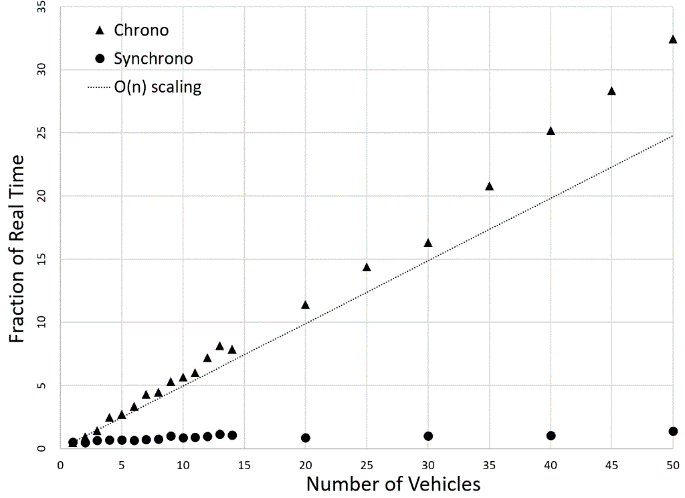
\includegraphics[width=0.8\columnwidth]{Figs/Syn-Chrono-Scaling.png}
	\caption{{\small Scaling comparison between \chrono{} and \synchrono{}. By running each simulation in parallel \synchrono{} handles scenarios with large numbers of vehicles much faster and closer to real-time than \chrono{}.}}   
	\label{fig:synchronoscalingold}
\end{figure}

\begin{figure}
	\centering
	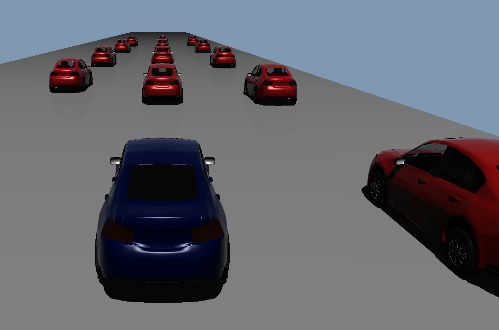
\includegraphics[width=0.8\columnwidth]{Figs/Syn-Platoon.png}
	\caption{{\small Image of a collection of agents in a shared, coherent virtual world.}}   
	\label{fig:synplatoonold}
\end{figure}

\subsection{ROS \chrono{} Control Interface}\label{s:roscontrolinterface}

To allow for the seamless testing of control algorithms that are intended to be easily transferred to real vehicles or robots, the toolset provides a \ros{} control interface that is exposed in \synchrono{}. Using \tcp{}, messages from \synchrono{} (i.e. sensor data packets), are sent into a \ros{} node on the same system running the vehicle control stack. This node also listens to the \ros{} control messages that are produced and sends them back to \synchrono{} for input to the \chrono{} agents. With this \ros{} interface, the tested control stack is independent of the \synchrono{} platform (i.e. can be run on a different operating system or architecture) and can be tested with inputs replicating those from reality, such as sensor and/or V2X communication data.

\clearpage

%% ============================================================
\section{Demonstration}\label{s:demonstration}
\todo[inline]{Asher's details on the proposed demonstration: the goal of the demonstration is to show a multi-agent simulation of vehicles driven with policies learned using RL in PyChrono. To accomplish this we will train a single agent to participate in a follow-the-leader convoy through a narrow path. It will be trained on rigid terrain until an optimal policy is found. We can then refine the policy on SCM terrain. The trained policy will be deployed for all vehicles in SynChrono. We can remove the need for sensing the SCM terrain if we using a simulated vehicle-to-vehicle message from the lead vehicle. I think it would be more interesting to include a camera as input and remove the need to know the position of the lead vehicle. Final decision on that TBD. The study will then be on how that policy is deployed in SynChrono and how it responds to perturbations in the form of ruts in the soil.}

\todo[inline]{DN - Training for convoy vehicle: sensor (GPS+Camera) fusion + rigid terrain + ghost vehicle(s). Training for lead vehicle: path (perhaps way points) + sensor fusion + obstacles}

\todo[inline]{DN: SynChrono scaling analysis on SCM with 1, 2, 4, 8, etc. vehicles; half going NS, half EW. SCM deformable terrain; deformable terrain shown in simulation and also picked up by sensor.}

%% ============================================================

\begin{figure}
    \centering
    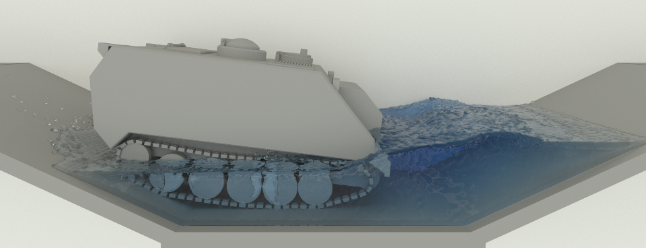
\includegraphics[width=0.8\columnwidth]{Figs/M113Fording.png}
    \caption{{\small M113 fording maneuver demonstrating \chrono{} and \chronomod{Vehicle} capabilities.}}   
    \label{fig:m113fording}
\end{figure}

\begin{figure}
    \centering
    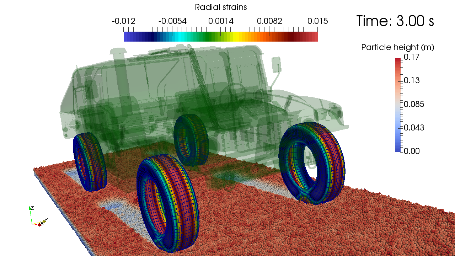
\includegraphics[width=0.8\columnwidth]{Figs/HMMWV-Granular.png}
    \caption{{\small HMMWV with flexible tires navigating granular terrain demonstrating vehicle dynamics, flexible body dynamics, and parallel computing support in \chrono{}.}}   
    \label{fig:hmmwvgranular}
\end{figure}

\begin{figure}
    \centering
    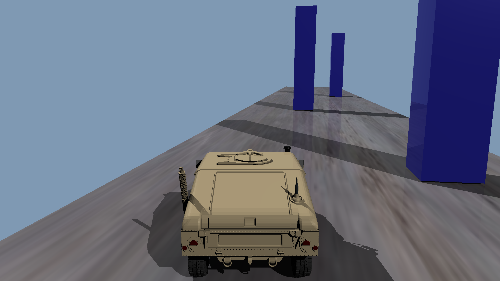
\includegraphics[width=0.8\columnwidth]{Figs/GymChrono-Pilars.png}
    \caption{{\small \gymchrono{}-enabled learning with simulated sensor data provided by \chronomod{Sensor} gradually allows the vehicle to understand how to avoid random obstacles placed in its path}}   
    \label{fig:gymchronopillars}
\end{figure}


This contribution outlines the current state of a BSD3 open-source simulation toolset whose goal is to assist practitioners in endowing autonomous agents with artificial intelligence; i.e., producing control strategies that enable heterogeneous teams of robots and wheeled/tracked vehicles to operate in off-road conditions in a coordinated fashion towards accomplishing a shared task. The toolset draws on: \chrono{} , which provides multi-physics support for agent modeling; \chronomod{Sensor}, which produces synthetic data for simulating sensing; \pychrono{} and \gymchrono{}, which provide support for machine learning; \synchrono{}, a software component for software/hardware/human in the loop studies that include multiple agents; and the \ros{}-\chrono{} Control Interface, which allows the toolset to converse with the software libraries/utilities provided by \ros{} . The reinforcement learning (RL) support provided through \gymchrono{} is demonstrated in conjunction with an RL experiment in which a HMMWV-type vehicle learns how to avoid road obstacles while moving in a convoy.


\section*{Acknowledgments}
This work was supported by a U.S. Army TARDEC project. \chrono{} development was supported in part by U.S. Army TARDEC Rapid Innovation Fund grant No. W911NF-13-R-0011, Topic No. 6a, ``Maneuverability Prediction''. 







%% *******************************************************************
%% Examples for including single- and double-column figures and tables
%% *******************************************************************

%\begin{figure}
%	\centering
%	\includegraphics[width=0.8\columnwidth]{Figs/hmmwv_1.png}
%	\caption{{\small A figure spanning a single column. The caption should wrap nicely here.}}   
%	\label{fig:one}
%\end{figure}

%\begin{figure*}
%	\centering
%	\includegraphics[width=0.75\textwidth]{Figs/hmmwv_1.png}
%	\caption{{\small A figure spanning the entire paper width}}    
%	\label{fig:two}
%\end{figure*}

% \begin{table}
% \begin{center}
% 	\begin{tabular}{||c |c | c||} 
% 		\hline
% 		Test  & Terrain  & Controller Vehicle \\
% 		Number &  Type & Model\\ [0.5ex] 	
% 		\hline\hline
% 		1 & Rigid & 2-DOF \\ 
% 		\hline
% 		2 & Rigid & 14-DOF \\
% 		\hline
% 		3 & Granular & 2-DOF \\
% 		\hline
% 		4 & Granular & 14-DOF \\
% 		\hline
% 	\end{tabular}
% \end{center}
% \caption{A table spanning a single column. The caption should wrap nicely here.}
% \label{t:one}
% \end{table}

% \begin{table*}
% 		\centering
% \begin{tabular}{ ||p{6cm}|p{1.8cm}|p{1.8cm}|p{1.8cm}|p{1.8cm}||  }
% 		\hline
% 		Test Number & 1 & 2 & 3 & 4\\
% 		\hline
% 		Controller Model & 2-DOF & 14-DOF & 2-DOF & 14-DOF\\
% 		\hline
% 		Terrain & Rigid & Rigid & Granular & Granular\\
% 		\hline
% 		Time to Target (s)  & 26.67 & 26.15 & 28.32 & 28.03\\ 
% 		\hline
% 		Minimum Obstacle Distance (m) & 0.897 & 5.462 & 3.491 & 4.721\\
% 		\hline
% 		Controller Effort & 0.0340 & 0.0340 & 0.0340 & 0.0306\\
% 		\hline
% 		Max. Lateral Acceleration (m/s$^{2}$)& 2.78 & 1.57 & 2.47 & 2.33 \\
% 		\hline
% 		Avg. Lateral Acceleration (m/s$^{2}$) &0.54 & 0.51 & 0.55 & 0.46\\
% 		\hline
% \end{tabular}
% \caption{A table spanning both columns.}
% \label{t:two}
% \end{table*}

%% ============================================================


\end{document}

